\documentclass[12pt]{article}
\usepackage[utf8]{inputenc}
\usepackage{amsmath,amsthm,amsfonts,amssymb}
\usepackage{tikz}
\usepackage{subfig}
\usepackage[english]{babel}
\usepackage{capt-of}
\usepackage{tabularray}
\newtheorem{theorem}{Theorem}
\usetikzlibrary{calc}
\usetikzlibrary{shapes}
\usepackage{hyperref}
%might be unnecessary
\usepackage{doi}

%bibliography CMDS

%\usepackage{cite}
%\usepackage[style=alphabetic]{biblatex}
%\bibliographystyle{plain}

%\usepackage[style=alphabetic]{biblatex}

% \usepackage[backend=biber,style=alphabetic]{biblatex}
\usepackage[backend=biber,style=numeric]{biblatex}
% \usepackage[backend=biber,style=abbrv]{biblatex}
% \usepackage[backend=biber,style=alpha]{biblatex}
%\usepackage[backend=bibtex,style=alphabetic]{biblatex}
\addbibresource{./bibb.bib}

%%% With amsthm package, creates environments for nicely formatted,
%%% labeled, and numbered propositions, etc.
\theoremstyle{plain}
\newtheorem{thm}{Theorem}
\newtheorem{lemma}[thm]{Lemma}
\newtheorem{prop}[thm]{Proposition}
\newtheorem{conj}[thm]{Conjecture}
\newtheorem{cor}[thm]{Corollary}
\newtheorem{claim}[thm]{Claim}
\newtheorem{fact}[thm]{Fact}
\newtheorem{constraint}[thm]{Constraint}

\theoremstyle{definition}
\newtheorem{eg}[thm]{Example}
\newtheorem{defn}[thm]{Definition}
\newtheorem{rem}[thm]{Remark}
\newtheorem{observ}[thm]{Observation}
\newtheorem{open}[thm]{Open Problem}
\newtheorem{prob.}[thm]{Problem}
\newtheorem{quest}[thm]{Question}

% I used these for making definitions and theorems, not what is above
\theoremstyle{remark}
\newtheorem{remark}[thm]{Remark}
\newtheorem{note}[thm]{Note}

\theoremstyle{definition}
\newtheorem{definition}{Definition}[section]
\newtheorem{exmp}{Example}[section]

%custom commands

% blank cell
\newcommand{\cell}[4]{ \draw[thick] ( #1 , #2 ) rectangle ( #3 , #4 );}

% invisible cell for spacing
\newcommand{\spacecell}[4]{ \draw[thick, color=white] ( #1 , #2 ) rectangle ( #3 , #4 );}

% open cell 
\newcommand{\cellopen}[4]{ \draw[thick] ( #1 , #2 ) rectangle ( #3 , #4 ); \node[shape=circle,draw=red,fill=red, inner sep=0pt,minimum size=3pt] (A) at ( #1 * 0.5 + #3 * 0.5 , #2 * 0.5 + #4 * 0.5 ){};}

% /
\newcommand{\cellA}[4]{ \draw[thick] ( #1 , #2 ) rectangle ( #3 , #4 ); \draw[red, thick, densely dotted] (#3 * 0.5 + #1 * 0.5 , #2) -- (#3, #4 * 0.5 + #2 * 0.5);}

% \
\newcommand{\cellB}[4]{ \draw[thick] ( #1 , #2 ) rectangle ( #3 , #4 ); \draw[red, thick, densely dotted] (#3 * 0.5 + #1 * 0.5 , #2) -- (#1, #4 * 0.5 + #2 * 0.5);}

% /
\newcommand{\cellC}[4]{ \draw[thick] ( #1 , #2 ) rectangle ( #3 , #4 ); \draw[red, thick, densely dotted] (#3 * 0.5 + #1 * 0.5 , #4) -- (#1, #4 * 0.5 + #2 * 0.5);}

% L
\newcommand{\cellD}[4]{ \draw[thick] ( #1 , #2 ) rectangle ( #3 , #4 ); \draw[red, thick, densely dotted] (#3 * 0.5 + #1 * 0.5 , #4) -- (#3, #4 * 0.5 + #2 * 0.5);}

% |
\newcommand{\cellE}[4]{ \draw[thick] ( #1 , #2 ) rectangle ( #3 , #4 ); \draw[red, thick, densely dotted] (#3 * 0.5 + #1 * 0.5 , #2) -- (#3 * 0.5 + #1 * 0.5 , #4);}

% -
\newcommand{\cellF}[4]{ \draw[thick] ( #1 , #2 ) rectangle ( #3 , #4 ); \draw[red, thick, densely dotted] (#3, #4 * 0.5 + #2 * 0.5) -- (#1, #4 * 0.5 + #2 * 0.5);}

\newcommand{\cellAf}[4]{\filldraw[gray!40] ( #1 , #2 ) rectangle ( #3 , #4 ); \draw[thick] ( #1 , #2 ) rectangle ( #3 , #4 ); \draw[red, thick, densely dotted] (#3 * 0.5 + #1 * 0.5 , #2) -- (#3, #4 * 0.5 + #2 * 0.5);}

% \
\newcommand{\cellBf}[4]{\filldraw[gray!40] ( #1 , #2 ) rectangle ( #3 , #4 ); \draw[thick] ( #1 , #2 ) rectangle ( #3 , #4 ); \draw[red, thick, densely dotted] (#3 * 0.5 + #1 * 0.5 , #2) -- (#1, #4 * 0.5 + #2 * 0.5);}

% /
\newcommand{\cellCf}[4]{\filldraw[gray!40] ( #1 , #2 ) rectangle ( #3 , #4 ); \draw[thick] ( #1 , #2 ) rectangle ( #3 , #4 ); \draw[red, thick, densely dotted] (#3 * 0.5 + #1 * 0.5 , #4) -- (#1, #4 * 0.5 + #2 * 0.5);}

% L
\newcommand{\cellDf}[4]{\filldraw[gray!40] ( #1 , #2 ) rectangle ( #3 , #4 ); \draw[thick] ( #1 , #2 ) rectangle ( #3 , #4 ); \draw[red, thick, densely dotted] (#3 * 0.5 + #1 * 0.5 , #4) -- (#3, #4 * 0.5 + #2 * 0.5);}

% |
\newcommand{\cellEf}[4]{\filldraw[gray!40] ( #1 , #2 ) rectangle ( #3 , #4 ); \draw[thick] ( #1 , #2 ) rectangle ( #3 , #4 ); \draw[red, thick, densely dotted] (#3 * 0.5 + #1 * 0.5 , #2) -- (#3 * 0.5 + #1 * 0.5 , #4);}

% -
\newcommand{\cellFf}[4]{\filldraw[gray!40] ( #1 , #2 ) rectangle ( #3 , #4 ); \draw[thick] ( #1 , #2 ) rectangle ( #3 , #4 ); \draw[red, thick, densely dotted] (#3, #4 * 0.5 + #2 * 0.5) -- (#1, #4 * 0.5 + #2 * 0.5);}


\newcommand{\lablnode}[3]{\node[shape=circle,draw=none,fill=none, inner sep=0pt,minimum size=5pt] (A) at ( #1 , #2 ) {#3};}

\newcommand{\lablvertex}[3]{\node[shape=circle,draw=none,fill=white, inner sep=2pt,minimum size=5pt] (A) at ( #1 , #2 ) {#3};}

\usepackage[margin=1in]{geometry}
\date{}
%doc info
% $\text{Hanke, Jack}^*$\\
% $\text{Schank, Richard}$\\
% $\text{Maltenfort, Michael}^*$
\author{
    \textbf{Jack Hanke}\\
    Northwestern University
    \and
    \textbf{Richard Schank}\\
    \and
    \textbf{Michael Maltenfort}\\
    Northwestern University
    }
\title{\textbf{Exact Enumeration of Polygon Mosaics}}
% \date{\today}

\begin{document}
\maketitle

\begin{center}

    \begin{abstract}
        Hong and Oh calculated upper and lower bounds on the number of polygon mosaics for $7$ distinct tiles that together model multiple ring polymers in physics. We exactly enumerate these polygon mosaics. The method we introduce generalizes to various other tile sets. We also introduce and enumerate a variation on polygon mosaics called messy polygon mosaics for various tile sets.
    \end{abstract}

\end{center}

\section{Introduction}

Consider the following set of $7$ symbols labelled $\{ T_1, \dots T_7 \}$ composed of unit squares and dotted lines connecting pairs of sides at their midpoints.

\begin{center}
    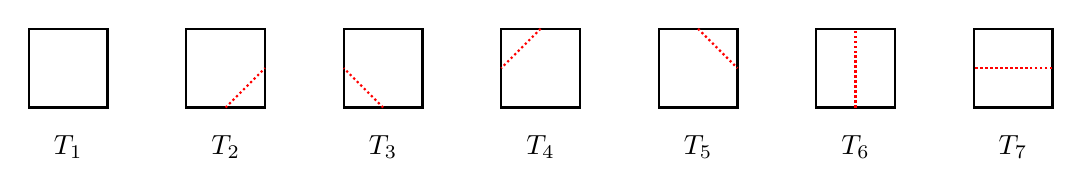
\begin{tikzpicture}
        \cell{-2}{0}{-1}{1}
        \( \lablnode{-1.5}{-0.5}{$T_1$} \) 
        \cellA{0}{0}{1}{1}
        \( \lablnode{0.5}{-0.5}{$T_2$} \) 
        \cellB{2}{0}{3}{1}
        \( \lablnode{2.5}{-0.5}{$T_3$} \) 
        \cellC{4}{0}{5}{1}
        \( \lablnode{4.5}{-0.5}{$T_4$} \) 
        \cellD{6}{0}{7}{1}
        \( \lablnode{6.5}{-0.5}{$T_5$} \) 
        \cellE{8}{0}{9}{1}
        \( \lablnode{8.5}{-0.5}{$T_6$} \) 
        \cellF{10}{0}{11}{1}
        \( \lablnode{10.5}{-0.5}{$T_7$} \) 
    \end{tikzpicture}
\end{center}

Call these symbols \textit{tiles}. A \textit{mosaic} of size $(m,n)$ is an $m \times n$ matrix of these tiles. For example, below is a mosaic of size $(5,7)$.

\begin{center}
    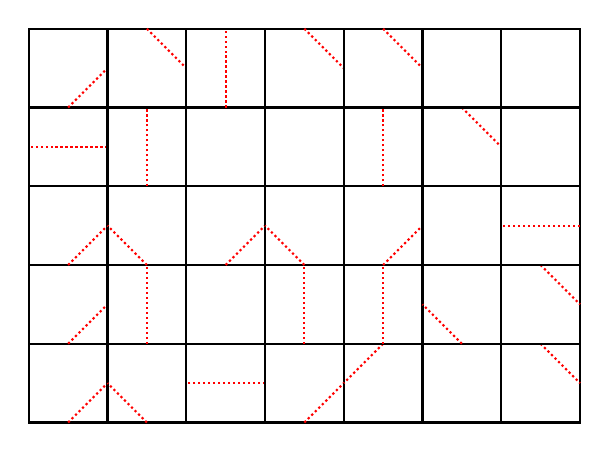
\begin{tikzpicture}
        % row1
        \cellA{0}{0}{1}{1}
        \cellB{1}{0}{2}{1}
        \cellF{2}{0}{3}{1}
        \cellA{3}{0}{4}{1}
        \cellC{4}{0}{5}{1}
        \cell{5}{0}{6}{1}
        \cellD{6}{0}{7}{1}
        % row2
        \cellA{0}{1}{1}{2}
        \cellE{1}{1}{2}{2}
        \cell{2}{1}{3}{2}
        \cellE{3}{1}{4}{2}
        \cellE{4}{1}{5}{2}
        \cellB{5}{1}{6}{2}
        \cellD{6}{1}{7}{2}
        % row3
        \cellA{0}{2}{1}{3}
        \cellB{1}{2}{2}{3}
        \cellA{2}{2}{3}{3}
        \cellB{3}{2}{4}{3}
        \cellA{4}{2}{5}{3}
        \cell{5}{2}{6}{3}
        \cellF{6}{2}{7}{3}
        % row4
        \cellF{0}{3}{1}{4}
        \cellE{1}{3}{2}{4}
        \cell{2}{3}{3}{4}
        \cell{3}{3}{4}{4}
        \cellE{4}{3}{5}{4}
        \cellD{5}{3}{6}{4}
        \cell{6}{3}{7}{4}
        % row5
        \cellA{0}{4}{1}{5}
        \cellD{1}{4}{2}{5}
        \cellE{2}{4}{3}{5}
        \cellD{3}{4}{4}{5}
        \cellD{4}{4}{5}{5}
        \cell{5}{4}{6}{5}
        \cell{6}{4}{7}{5}
\end{tikzpicture}
\end{center}

Consider a edge shared between two tiles in the above figure. The edge has either $0$, $1$, or $2$ dotted lines drawn from its midpoint. Also note that the edges of the tiles on the boundary of the matrix are not shared by another tile. Therefore these edges only have $0$ or $1$ dotted lines drawn from their midpoint. We define a \textit{polygon mosaic} to be a mosaic that has all unit edges having $0$ or $2$ dotted lines drawn from their midpoint.

We call these polygon mosaics because, other than the mosaic consisting of all $T_1$ tiles, the dotted lines form shapes we call \textit{polygons}\footnote{Polygons are more commonly called "self-avoiding polygons" in the literature to emphasize their relationship with self-avoiding walks.}. 

\begin{exmp}
\label{exmp: clean sap}
Below is an example of a polygon mosaic of size $(5,7)$ that contains $2$ polygons, with the squares that make them up hilighted in gray.

\begin{center}
    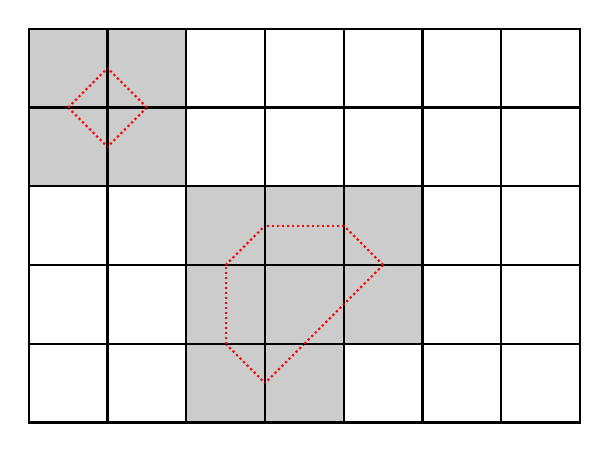
\begin{tikzpicture}
        % row1
        \cell{0}{0}{1}{1}
        \cell{1}{0}{2}{1}
        \cellDf{2}{0}{3}{1}
        \cellCf{3}{0}{4}{1}
        \cell{4}{0}{5}{1}
        \cell{5}{0}{6}{1}
        \cell{6}{0}{7}{1}
        % row2
        \cell{0}{1}{1}{2}
        \cell{1}{1}{2}{2}
        \cellEf{2}{1}{3}{2}
        \cellAf{3}{1}{4}{2}
        \cellCf{4}{1}{5}{2}
        \cell{5}{1}{6}{2}
        \cell{6}{1}{7}{2}
        % row3
        \cell{0}{2}{1}{3}
        \cell{1}{2}{2}{3}
        \cellAf{2}{2}{3}{3}
        \cellFf{3}{2}{4}{3}
        \cellBf{4}{2}{5}{3}
        \cell{5}{2}{6}{3}
        \cell{6}{2}{7}{3}
        % row4
        \cellDf{0}{3}{1}{4}
        \cellCf{1}{3}{2}{4}
        \cell{2}{3}{3}{4}
        \cell{3}{3}{4}{4}
        \cell{4}{3}{5}{4}
        \cell{5}{3}{6}{4}
        \cell{6}{3}{7}{4}
        % row5
        \cellAf{0}{4}{1}{5}
        \cellBf{1}{4}{2}{5}
        \cell{2}{4}{3}{5}
        \cell{3}{4}{4}{5}
        \cell{4}{4}{5}{5}
        \cell{5}{4}{6}{5}
        \cell{6}{4}{7}{5}
    \end{tikzpicture}
\end{center}
\end{exmp}

Note that in large enough mosaics, it is possible for larger polygons to surround smaller polygons. 

Let $p_{m,n}$ be the number of polygon mosaics of size $(m,n)$. First notice that if either $m$ or $n$ is $1$, one cannot construct a polygon mosaic, so 
$$p_{m,1} = p_{1,n} = 0.$$

Hong and Oh \cite[Hong2018]{Hong2018} gave the following upper and lower bounds\footnote{The authors did not consider the mosaic containing all $T_1$ tiles a polygon mosaic, and so define $p_{m,n}$ as one less than what we define.} for $m,n \geq 2$. 

$$2^{m+n-3} \left(\frac{17}{10}\right)^{(m-2)(n-2)} \leq p_{m,n} \leq 2^{m+n-3} \left(\frac{31}{16}\right)^{(m-2)(n-2)}.$$

In Theorem \ref{thm: main theorem}, we provide an exact expression for $p_{m,n}$ for $m,n \geq 2$. We also introduce messy polygon mosaics—a variant of polygon mosaics—and enumerate them using a similar strategy.

First we define $A(m) \in \mathbb{Z}^{2^{m-1} \times 2^{m-1}}$, which we use to enumerate $p_{m,n}$.

\begin{defn}
\label{defn: A}

First define $A(2) = \begin{bmatrix}
1 & 1 \\
1 & 1
\end{bmatrix}
$. We recursively define $A(k+1)$ given $A(k)$. Begin by writing
$
A(k) = \begin{bmatrix}
A_{0,0} & A_{0,1} \\
A_{1,0} & A_{1,1}
\end{bmatrix}
$, where the block matrices $A_{i,j}$ are square block matrices of size $2^{k-2} \times 2^{k-2}$. We then have

$$
A(k+1) = \begin{bmatrix}
A_{0,0} & A_{0,0} & A_{0,1} & A_{0,1} \\
A_{0,0} & A_{0,0} & 0A_{0,1} & A_{0,1} \\
A_{1,0} & 0A_{1,0} & A_{1,1} & A_{1,1} \\
A_{1,0} & A_{1,0} & A_{1,1} & A_{1,1} \\
\end{bmatrix},
$$

Construct $A(m)$ by starting with $k=2$ and recursing until $k=m$. 

\end{defn}

\begin{thm}
\label{thm: main theorem}    
The number of polygon mosaics $p_{m,n}$ is the $(0,0)$-th entry of $A(m)^n$.
\end{thm}

\section{Proof of Theorem \ref{thm: main theorem}}

\begin{proof}

For a given mosaic, label the vertices of the tiles as follows. If the vertex is surrounded by an even number of polygons, label it $0$. If the vertex is surrounded by an odd number of polygons, label it $1$. To make a \textit{vertex labeling} we also remove the dotted lines from all tiles in the mosaic. Using the mosaic from Example \ref{exmp: clean sap}, we show both the labeling of the vertices, and then the removal of the dotted lines.

\begin{center}
    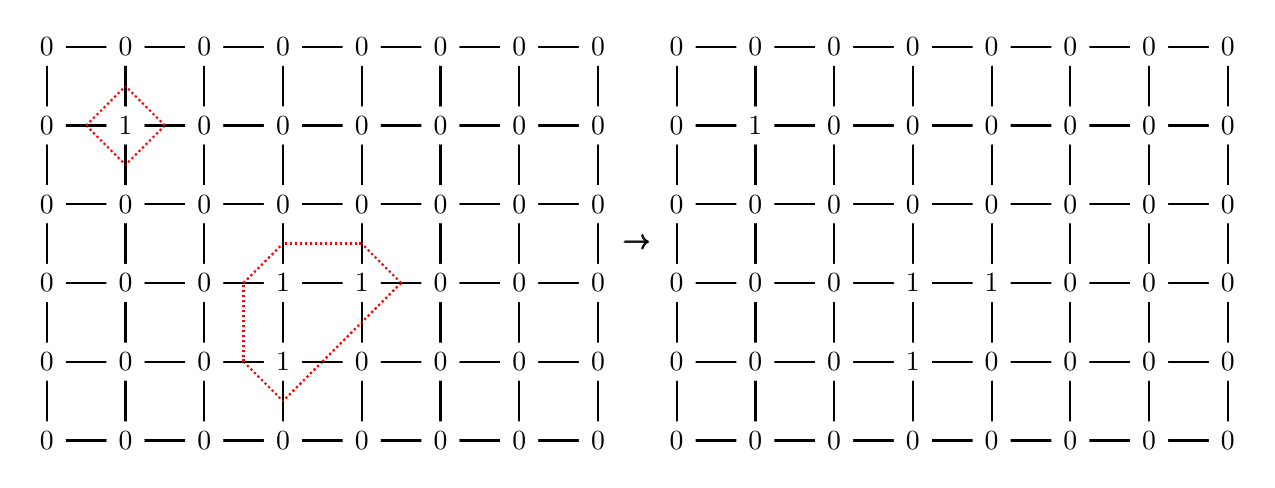
\begin{tikzpicture}
        % row1
        \cell{0}{0}{1}{1}
        \cell{1}{0}{2}{1}
        \cellD{2}{0}{3}{1}
        \cellC{3}{0}{4}{1}
        \cell{4}{0}{5}{1}
        \cell{5}{0}{6}{1}
        \cell{6}{0}{7}{1}
        % row2
        \cell{0}{1}{1}{2}
        \cell{1}{1}{2}{2}
        \cellE{2}{1}{3}{2}
        \cellA{3}{1}{4}{2}
        \cellC{4}{1}{5}{2}
        \cell{5}{1}{6}{2}
        \cell{6}{1}{7}{2}
        % row3
        \cell{0}{2}{1}{3}
        \cell{1}{2}{2}{3}
        \cellA{2}{2}{3}{3}
        \cellF{3}{2}{4}{3}
        \cellB{4}{2}{5}{3}
        \cell{5}{2}{6}{3}
        \cell{6}{2}{7}{3}
        % row4
        \cellD{0}{3}{1}{4}
        \cellC{1}{3}{2}{4}
        \cell{2}{3}{3}{4}
        \cell{3}{3}{4}{4}
        \cell{4}{3}{5}{4}
        \cell{5}{3}{6}{4}
        \cell{6}{3}{7}{4}
        % row5
        \cellA{0}{4}{1}{5}
        \cellB{1}{4}{2}{5}
        \cell{2}{4}{3}{5}
        \cell{3}{4}{4}{5}
        \cell{4}{4}{5}{5}
        \cell{5}{4}{6}{5}
        \cell{6}{4}{7}{5}
        % label for row1
        \( \lablvertex{0}{0}{$0$} \)
        \( \lablvertex{1}{0}{$0$} \)
        \( \lablvertex{2}{0}{$0$} \)
        \( \lablvertex{3}{0}{$0$} \)
        \( \lablvertex{4}{0}{$0$} \)
        \( \lablvertex{5}{0}{$0$} \)
        \( \lablvertex{6}{0}{$0$} \)
        \( \lablvertex{7}{0}{$0$} \)
        % label for row1
        \( \lablvertex{0}{1}{$0$} \)
        \( \lablvertex{1}{1}{$0$} \)
        \( \lablvertex{2}{1}{$0$} \)
        \( \lablvertex{3}{1}{$1$} \)
        \( \lablvertex{4}{1}{$0$} \)
        \( \lablvertex{5}{1}{$0$} \)
        \( \lablvertex{6}{1}{$0$} \)
        \( \lablvertex{7}{1}{$0$} \)
        % label for row1
        \( \lablvertex{0}{2}{$0$} \)
        \( \lablvertex{1}{2}{$0$} \)
        \( \lablvertex{2}{2}{$0$} \)
        \( \lablvertex{3}{2}{$1$} \)
        \( \lablvertex{4}{2}{$1$} \)
        \( \lablvertex{5}{2}{$0$} \)
        \( \lablvertex{6}{2}{$0$} \)
        \( \lablvertex{7}{2}{$0$} \)
        % label for row1
        \( \lablvertex{0}{3}{$0$} \)
        \( \lablvertex{1}{3}{$0$} \)
        \( \lablvertex{2}{3}{$0$} \)
        \( \lablvertex{3}{3}{$0$} \)
        \( \lablvertex{4}{3}{$0$} \)
        \( \lablvertex{5}{3}{$0$} \)
        \( \lablvertex{6}{3}{$0$} \)
        \( \lablvertex{7}{3}{$0$} \)
        % label for row1
        \( \lablvertex{0}{4}{$0$} \)
        \( \lablvertex{1}{4}{$1$} \)
        \( \lablvertex{2}{4}{$0$} \)
        \( \lablvertex{3}{4}{$0$} \)
        \( \lablvertex{4}{4}{$0$} \)
        \( \lablvertex{5}{4}{$0$} \)
        \( \lablvertex{6}{4}{$0$} \)
        \( \lablvertex{7}{4}{$0$} \)
        % label for row1
        \( \lablvertex{0}{5}{$0$} \)
        \( \lablvertex{1}{5}{$0$} \)
        \( \lablvertex{2}{5}{$0$} \)
        \( \lablvertex{3}{5}{$0$} \)
        \( \lablvertex{4}{5}{$0$} \)
        \( \lablvertex{5}{5}{$0$} \)
        \( \lablvertex{6}{5}{$0$} \)
        \( \lablvertex{7}{5}{$0$} \)
        % arrow
        \( \lablnode{7.5}{2.5}{$\pmb{\to}$} \)

        % row1
        \cell{8}{0}{9}{1}
        \cell{9}{0}{10}{1}
        \cell{10}{0}{11}{1}
        \cell{11}{0}{12}{1}
        \cell{12}{0}{13}{1}
        \cell{13}{0}{14}{1}
        \cell{14}{0}{15}{1}
        % row2
        \cell{8}{1}{9}{2}
        \cell{9}{1}{10}{2}
        \cell{10}{1}{11}{2}
        \cell{11}{1}{12}{2}
        \cell{12}{1}{13}{2}
        \cell{13}{1}{14}{2}
        \cell{14}{1}{15}{2}
        % row3
        \cell{8}{2}{9}{3}
        \cell{9}{2}{10}{3}
        \cell{10}{2}{11}{3}
        \cell{11}{2}{12}{3}
        \cell{12}{2}{13}{3}
        \cell{13}{2}{14}{3}
        \cell{14}{2}{15}{3}
        % row4
        \cell{8}{3}{9}{4}
        \cell{9}{3}{10}{4}
        \cell{10}{3}{11}{4}
        \cell{11}{3}{12}{4}
        \cell{12}{3}{13}{4}
        \cell{13}{3}{14}{4}
        \cell{14}{3}{15}{4}
        % row5
        \cell{8}{4}{9}{5}
        \cell{9}{4}{10}{5}
        \cell{10}{4}{11}{5}
        \cell{11}{4}{12}{5}
        \cell{12}{4}{13}{5}
        \cell{13}{4}{14}{5}
        \cell{14}{4}{15}{5}

        % label for row1
        \( \lablvertex{8}{0}{$0$} \)
        \( \lablvertex{9}{0}{$0$} \)
        \( \lablvertex{10}{0}{$0$} \)
        \( \lablvertex{11}{0}{$0$} \)
        \( \lablvertex{12}{0}{$0$} \)
        \( \lablvertex{13}{0}{$0$} \)
        \( \lablvertex{14}{0}{$0$} \)
        \( \lablvertex{15}{0}{$0$} \)
        % label for row1
        \( \lablvertex{8}{1}{$0$} \)
        \( \lablvertex{9}{1}{$0$} \)
        \( \lablvertex{10}{1}{$0$} \)
        \( \lablvertex{11}{1}{$1$} \)
        \( \lablvertex{12}{1}{$0$} \)
        \( \lablvertex{13}{1}{$0$} \)
        \( \lablvertex{14}{1}{$0$} \)
        \( \lablvertex{15}{1}{$0$} \)
        % label for row1
        \( \lablvertex{8}{2}{$0$} \)
        \( \lablvertex{9}{2}{$0$} \)
        \( \lablvertex{10}{2}{$0$} \)
        \( \lablvertex{11}{2}{$1$} \)
        \( \lablvertex{12}{2}{$1$} \)
        \( \lablvertex{13}{2}{$0$} \)
        \( \lablvertex{14}{2}{$0$} \)
        \( \lablvertex{15}{2}{$0$} \)
        % label for row1
        \( \lablvertex{8}{3}{$0$} \)
        \( \lablvertex{9}{3}{$0$} \)
        \( \lablvertex{10}{3}{$0$} \)
        \( \lablvertex{11}{3}{$0$} \)
        \( \lablvertex{12}{3}{$0$} \)
        \( \lablvertex{13}{3}{$0$} \)
        \( \lablvertex{14}{3}{$0$} \)
        \( \lablvertex{15}{3}{$0$} \)
        % label for row1
        \( \lablvertex{8}{4}{$0$} \)
        \( \lablvertex{9}{4}{$1$} \)
        \( \lablvertex{10}{4}{$0$} \)
        \( \lablvertex{11}{4}{$0$} \)
        \( \lablvertex{12}{4}{$0$} \)
        \( \lablvertex{13}{4}{$0$} \)
        \( \lablvertex{14}{4}{$0$} \)
        \( \lablvertex{15}{4}{$0$} \)
        % label for row1
        \( \lablvertex{8}{5}{$0$} \)
        \( \lablvertex{9}{5}{$0$} \)
        \( \lablvertex{10}{5}{$0$} \)
        \( \lablvertex{11}{5}{$0$} \)
        \( \lablvertex{12}{5}{$0$} \)
        \( \lablvertex{13}{5}{$0$} \)
        \( \lablvertex{14}{5}{$0$} \)
        \( \lablvertex{15}{5}{$0$} \)

    \end{tikzpicture}
\end{center}

The critical point is this: even with the dotted lines removed, the vertex labeling uniquely identifies the polygon mosaic. This is true even if there are polygons surrounding other polygons. This is because the vertex labeling of an individual cell, which we will call a \textit{cell-labeling}, uniquely corresponds with a cell $T_i$. This is shown below.

\begin{center}
    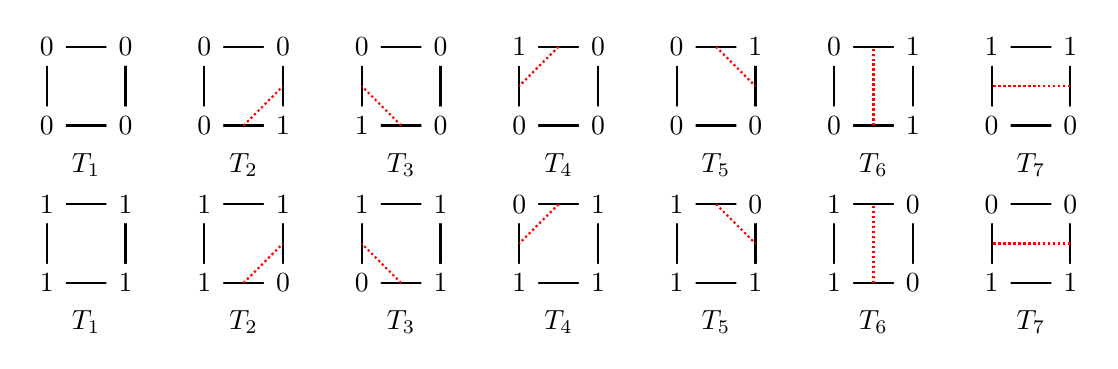
\begin{tikzpicture}
        % row 1
        \cell{-2}{0}{-1}{1}
        \( \lablnode{-1.5}{-0.5}{$T_1$} \) 
        \cellA{0}{0}{1}{1}
        \( \lablnode{0.5}{-0.5}{$T_2$} \) 
        \cellB{2}{0}{3}{1}
        \( \lablnode{2.5}{-0.5}{$T_3$} \) 
        \cellC{4}{0}{5}{1}
        \( \lablnode{4.5}{-0.5}{$T_4$} \) 
        \cellD{6}{0}{7}{1}
        \( \lablnode{6.5}{-0.5}{$T_5$} \) 
        \cellE{8}{0}{9}{1}
        \( \lablnode{8.5}{-0.5}{$T_6$} \) 
        \cellF{10}{0}{11}{1}
        \( \lablnode{10.5}{-0.5}{$T_7$} \) 

        \( \lablvertex{-2}{0}{$1$} \)
        \( \lablvertex{-2}{1}{$1$} \)
        \( \lablvertex{-1}{0}{$1$} \)
        \( \lablvertex{-1}{1}{$1$} \)

        \( \lablvertex{0}{0}{$1$} \)
        \( \lablvertex{0}{1}{$1$} \)
        \( \lablvertex{1}{0}{$0$} \)
        \( \lablvertex{1}{1}{$1$} \)

        \( \lablvertex{2}{0}{$0$} \)
        \( \lablvertex{2}{1}{$1$} \)
        \( \lablvertex{3}{0}{$1$} \)
        \( \lablvertex{3}{1}{$1$} \)

        \( \lablvertex{4}{0}{$1$} \)
        \( \lablvertex{4}{1}{$0$} \)
        \( \lablvertex{5}{0}{$1$} \)
        \( \lablvertex{5}{1}{$1$} \)

        \( \lablvertex{6}{0}{$1$} \)
        \( \lablvertex{6}{1}{$1$} \)
        \( \lablvertex{7}{0}{$1$} \)
        \( \lablvertex{7}{1}{$0$} \)

        \( \lablvertex{8}{0}{$1$} \)
        \( \lablvertex{8}{1}{$1$} \)
        \( \lablvertex{9}{0}{$0$} \)
        \( \lablvertex{9}{1}{$0$} \)

        \( \lablvertex{10}{0}{$1$} \)
        \( \lablvertex{10}{1}{$0$} \)
        \( \lablvertex{11}{0}{$1$} \)
        \( \lablvertex{11}{1}{$0$} \)


        % row 2
        \cell{-2}{2}{-1}{3}
        \( \lablnode{-1.5}{1.5}{$T_1$} \) 
        \cellA{0}{2}{1}{3}
        \( \lablnode{0.5}{1.5}{$T_2$} \) 
        \cellB{2}{2}{3}{3}
        \( \lablnode{2.5}{1.5}{$T_3$} \) 
        \cellC{4}{2}{5}{3}
        \( \lablnode{4.5}{1.5}{$T_4$} \) 
        \cellD{6}{2}{7}{3}
        \( \lablnode{6.5}{1.5}{$T_5$} \) 
        \cellE{8}{2}{9}{3}
        \( \lablnode{8.5}{1.5}{$T_6$} \) 
        \cellF{10}{2}{11}{3}
        \( \lablnode{10.5}{1.5}{$T_7$} \) 


        \( \lablvertex{-2}{2}{$0$} \)
        \( \lablvertex{-2}{3}{$0$} \)
        \( \lablvertex{-1}{2}{$0$} \)
        \( \lablvertex{-1}{3}{$0$} \)

        \( \lablvertex{0}{2}{$0$} \)
        \( \lablvertex{0}{3}{$0$} \)
        \( \lablvertex{1}{2}{$1$} \)
        \( \lablvertex{1}{3}{$0$} \)

        \( \lablvertex{2}{2}{$1$} \)
        \( \lablvertex{2}{3}{$0$} \)
        \( \lablvertex{3}{2}{$0$} \)
        \( \lablvertex{3}{3}{$0$} \)

        \( \lablvertex{4}{2}{$0$} \)
        \( \lablvertex{4}{3}{$1$} \)
        \( \lablvertex{5}{2}{$0$} \)
        \( \lablvertex{5}{3}{$0$} \)

        \( \lablvertex{6}{2}{$0$} \)
        \( \lablvertex{6}{3}{$0$} \)
        \( \lablvertex{7}{2}{$0$} \)
        \( \lablvertex{7}{3}{$1$} \)

        \( \lablvertex{8}{2}{$0$} \)
        \( \lablvertex{8}{3}{$0$} \)
        \( \lablvertex{9}{2}{$1$} \)
        \( \lablvertex{9}{3}{$1$} \)

        \( \lablvertex{10}{2}{$0$} \)
        \( \lablvertex{10}{3}{$1$} \)
        \( \lablvertex{11}{2}{$0$} \)
        \( \lablvertex{11}{3}{$1$} \)
    \end{tikzpicture}
\end{center}

We can then enumerate $p_{m,n}$ by enumerating the number of vertex labelings that correspond with a valid polygon mosaic. 

Consider the collection of vertex labelings for a $m \times n$ grid of cells. To correspond with a polygon mosaic, each boundary vertex is necessarily labelled $0$, and each interior vertex is labelled $0$ or $1$. Additionally, of these $2^{(m-1)(n-1)}$ labelings, the labelings that correspond with valid polygon mosaics are ones that do not contain the following two cell-labelings.

\begin{center}
    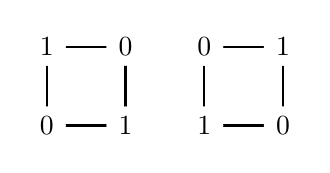
\begin{tikzpicture}
        % row1
        \cell{0}{0}{1}{1}
        \cell{2}{0}{3}{1}

        \( \lablvertex{0}{0}{$0$} \)
        \( \lablvertex{0}{1}{$1$} \)
        \( \lablvertex{1}{0}{$1$} \)
        \( \lablvertex{1}{1}{$0$} \)

        \( \lablvertex{2}{0}{$1$} \)
        \( \lablvertex{2}{1}{$0$} \)
        \( \lablvertex{3}{0}{$0$} \)
        \( \lablvertex{3}{1}{$1$} \)
        
    \end{tikzpicture}
\end{center}

These two cell-labelings aren't associated with any of the cells $T_1, \dots, T_7$, and so cannot correspond with a polygon mosaic. We seek a recursive solution to enumerate the number of vertex labelings for a $m \times n$ grid with these  conditions: the labeling has a boundary of all $0$'s and does not contain the above cell-labelings. 

Our solution accomplishes this by building $m \times n$ vertex labelings for fixed $m$ using vertex labelings of $m \times 1$ columns of cells. These columns have vertex labelings such that the top and bottom edge all labelled $0$. One of these columns for $m=3$ is below.

\begin{center}
    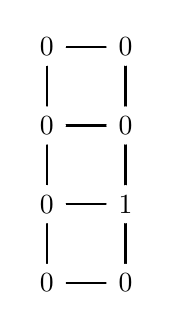
\begin{tikzpicture}
        \cell{0}{0}{1}{1}
        \cell{0}{1}{1}{2}
        \cell{0}{2}{1}{3}

        % col 1
        \( \lablvertex{0}{0}{$0$} \)
        \( \lablvertex{0}{1}{$0$} \)
        \( \lablvertex{0}{2}{$0$} \)
        \( \lablvertex{0}{3}{$0$} \)
        
        % col 2
        \( \lablvertex{1}{0}{$0$} \)
        \( \lablvertex{1}{1}{$1$} \)
        \( \lablvertex{1}{2}{$0$} \)
        \( \lablvertex{1}{3}{$0$} \)
        
        % index
        % \( \lablnode{0.5}{-1}{$(0,2)$} \)
    \end{tikzpicture}
\end{center}

It is useful to define an index for vertex labelings of these $m \times 1$ columns. To do this, consider reading a column of vertex labelings from bottom to top, ignoring the first and last $0$'s. If we interpret these sequences for the left and right column as binary numbers $b_{left}$ and $b_{right}$, the index in base ten is the pair $(b_{left}, b_{right})$. For example, for the above $m=3$ column, we have sequences $00$ for the left column and $10$ for the right column, so the index is $(0,2)$.

Next consider a column with index $(0, b_{1})$ for some $b_{1} \in [0,2^{m-1}-1]$. For reasons we will see later, let's call this the \textit{starting column}. Now consider appending a column with index $(b_{1}, b_{2})$ for some $b_{2} \in [0,2^{m-1}-1]$. For example, below is a diagram for appending our starting column $(0,2)$ with column $(2,3)$. 

\begin{center}
    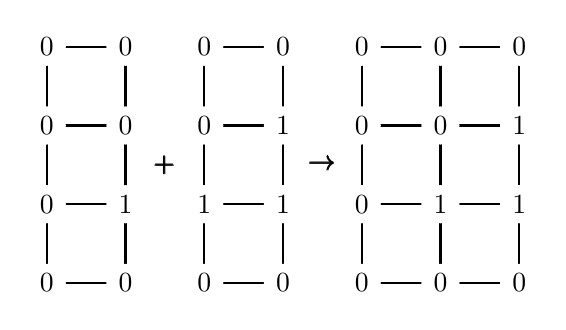
\begin{tikzpicture}
        \cell{0}{0}{1}{1}
        \cell{0}{1}{1}{2}
        \cell{0}{2}{1}{3}
        % col 1
        \( \lablvertex{0}{0}{$0$} \)
        \( \lablvertex{0}{1}{$0$} \)
        \( \lablvertex{0}{2}{$0$} \)
        \( \lablvertex{0}{3}{$0$} \)
        % col 2
        \( \lablvertex{1}{0}{$0$} \)
        \( \lablvertex{1}{1}{$1$} \)
        \( \lablvertex{1}{2}{$0$} \)
        \( \lablvertex{1}{3}{$0$} \)

        % plus
        \( \lablnode{1.5}{1.5}{$\pmb{+}$} \)

        \cell{2}{0}{3}{1}
        \cell{2}{1}{3}{2}
        \cell{2}{2}{3}{3}
        % col 1
        \( \lablvertex{2}{0}{$0$} \)
        \( \lablvertex{2}{1}{$1$} \)
        \( \lablvertex{2}{2}{$0$} \)
        \( \lablvertex{2}{3}{$0$} \)
        % col 1
        \( \lablvertex{3}{0}{$0$} \)
        \( \lablvertex{3}{1}{$1$} \)
        \( \lablvertex{3}{2}{$1$} \)
        \( \lablvertex{3}{3}{$0$} \)

        \( \lablnode{3.5}{1.5}{$\pmb{\to}$} \)

        \cell{4}{0}{5}{1}
        \cell{4}{1}{5}{2}
        \cell{4}{2}{5}{3}
        \cell{5}{0}{6}{1}
        \cell{5}{1}{6}{2}
        \cell{5}{2}{6}{3}

        % col 1
        \( \lablvertex{4}{0}{$0$} \)
        \( \lablvertex{4}{1}{$0$} \)
        \( \lablvertex{4}{2}{$0$} \)
        \( \lablvertex{4}{3}{$0$} \)
        % col 2
        \( \lablvertex{5}{0}{$0$} \)
        \( \lablvertex{5}{1}{$1$} \)
        \( \lablvertex{5}{2}{$0$} \)
        \( \lablvertex{5}{3}{$0$} \)
        % col 3
        \( \lablvertex{6}{0}{$0$} \)
        \( \lablvertex{6}{1}{$1$} \)
        \( \lablvertex{6}{2}{$1$} \)
        \( \lablvertex{6}{3}{$0$} \)


    \end{tikzpicture}
\end{center}

Notice that in the above example we have created a vertex labeling for an $m \times 2$ grid of cells, in which the left-most vertex column labels are all $0$ (left index of $0$). Also note that we did not create either illegal cell-labelings with column $(2,3)$. However, we could append the column $(2,1)$, which would create an illegal cell-labeling. 

Finally, if we further appended a column with label $(b_2,0)$, we would have created a vertex labeling with a boundary of all $0$'s. For this reason, let's call a column with index $(b,0)$ for $b \in [0,2^{m-1}-1]$ an \textit{ending column}. This vertex labeling would correspond with $1$ polygon mosaic if the middle column had index $(2,3)$, but not if the middle column had index $(2,1)$.

This motivates the creation of a matrix $A(m)$ to every column index $(i,j)$, where $A(m)_{i,j}=1$ if the column labeling corresponds with a legal polygon mosaic, and $0$ otherwise. For example, the $A(3)$ matrix corresponds with the following labeled columns. 

\begin{center}
    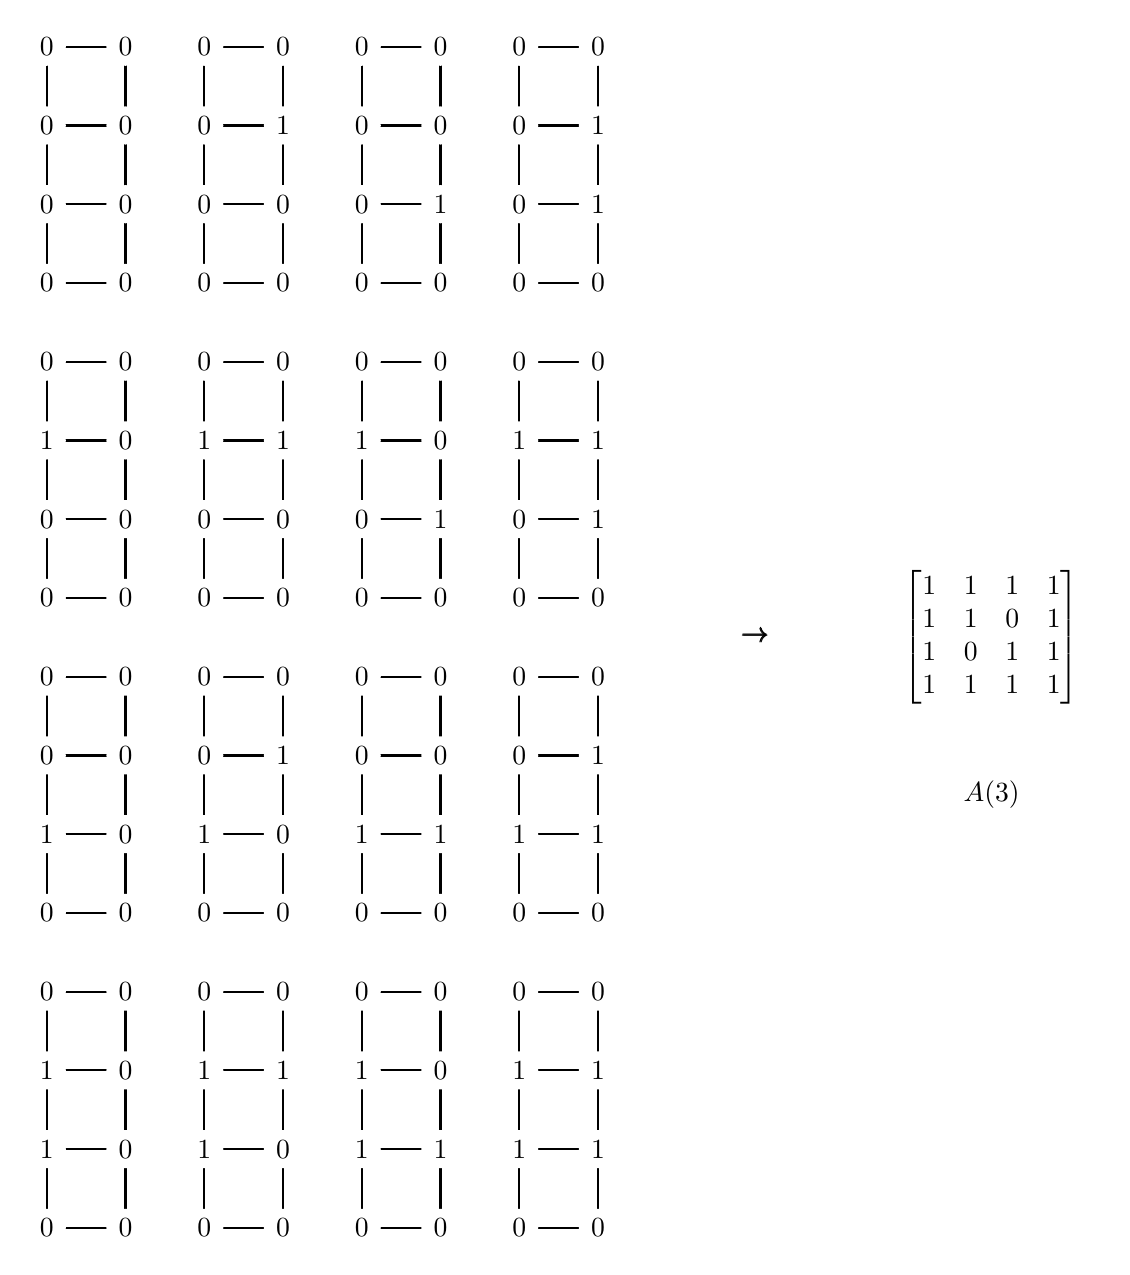
\begin{tikzpicture}
        % row1
        \cell{0}{0}{1}{1}
        \cell{0}{1}{1}{2}
        \cell{0}{2}{1}{3}

        \cell{2}{0}{3}{1}
        \cell{2}{1}{3}{2}
        \cell{2}{2}{3}{3}

        \cell{4}{0}{5}{1}
        \cell{4}{1}{5}{2}
        \cell{4}{2}{5}{3}

        \cell{6}{0}{7}{1}
        \cell{6}{1}{7}{2}
        \cell{6}{2}{7}{3}
        % row2
        \cell{0}{4}{1}{5}
        \cell{0}{5}{1}{6}
        \cell{0}{6}{1}{7}

        \cell{2}{4}{3}{5}
        \cell{2}{5}{3}{6}
        \cell{2}{6}{3}{7}

        \cell{4}{4}{5}{5}
        \cell{4}{5}{5}{6}
        \cell{4}{6}{5}{7}

        \cell{6}{4}{7}{5}
        \cell{6}{5}{7}{6}
        \cell{6}{6}{7}{7}
        % row3
        \cell{0}{8}{1}{9}
        \cell{0}{9}{1}{10}
        \cell{0}{10}{1}{11}

        \cell{2}{8}{3}{9}
        \cell{2}{9}{3}{10}
        \cell{2}{10}{3}{11}

        \cell{4}{8}{5}{9}
        \cell{4}{9}{5}{10}
        \cell{4}{10}{5}{11}

        \cell{6}{8}{7}{9}
        \cell{6}{9}{7}{10}
        \cell{6}{10}{7}{11}
        % row4
        \cell{0}{12}{1}{13}
        \cell{0}{13}{1}{14}
        \cell{0}{14}{1}{15}

        \cell{2}{12}{3}{13}
        \cell{2}{13}{3}{14}
        \cell{2}{14}{3}{15}

        \cell{4}{12}{5}{13}
        \cell{4}{13}{5}{14}
        \cell{4}{14}{5}{15}

        \cell{6}{12}{7}{13}
        \cell{6}{13}{7}{14}
        \cell{6}{14}{7}{15}
        % row 1
        \( \lablvertex{0}{0}{$0$} \)
        \( \lablvertex{0}{1}{$1$} \)
        \( \lablvertex{0}{2}{$1$} \)
        \( \lablvertex{0}{3}{$0$} \)
        
        \( \lablvertex{1}{0}{$0$} \)
        \( \lablvertex{1}{1}{$0$} \)
        \( \lablvertex{1}{2}{$0$} \)
        \( \lablvertex{1}{3}{$0$} \)
        
        \( \lablvertex{2}{0}{$0$} \)
        \( \lablvertex{2}{1}{$1$} \)
        \( \lablvertex{2}{2}{$1$} \)
        \( \lablvertex{2}{3}{$0$} \)
        
        \( \lablvertex{3}{0}{$0$} \)
        \( \lablvertex{3}{1}{$0$} \)
        \( \lablvertex{3}{2}{$1$} \)
        \( \lablvertex{3}{3}{$0$} \)
        
        \( \lablvertex{4}{0}{$0$} \)
        \( \lablvertex{4}{1}{$1$} \)
        \( \lablvertex{4}{2}{$1$} \)
        \( \lablvertex{4}{3}{$0$} \)
        
        \( \lablvertex{5}{0}{$0$} \)
        \( \lablvertex{5}{1}{$1$} \)
        \( \lablvertex{5}{2}{$0$} \)
        \( \lablvertex{5}{3}{$0$} \)
        
        \( \lablvertex{6}{0}{$0$} \)
        \( \lablvertex{6}{1}{$1$} \)
        \( \lablvertex{6}{2}{$1$} \)
        \( \lablvertex{6}{3}{$0$} \)
        
        \( \lablvertex{7}{0}{$0$} \)
        \( \lablvertex{7}{1}{$1$} \)
        \( \lablvertex{7}{2}{$1$} \)
        \( \lablvertex{7}{3}{$0$} \)
        % row 2
        \( \lablvertex{0}{4}{$0$} \)
        \( \lablvertex{0}{5}{$1$} \)
        \( \lablvertex{0}{6}{$0$} \)
        \( \lablvertex{0}{7}{$0$} \)
        
        \( \lablvertex{1}{4}{$0$} \)
        \( \lablvertex{1}{5}{$0$} \)
        \( \lablvertex{1}{6}{$0$} \)
        \( \lablvertex{1}{7}{$0$} \)
        
        \( \lablvertex{2}{4}{$0$} \)
        \( \lablvertex{2}{5}{$1$} \)
        \( \lablvertex{2}{6}{$0$} \)
        \( \lablvertex{2}{7}{$0$} \)
        
        \( \lablvertex{3}{4}{$0$} \)
        \( \lablvertex{3}{5}{$0$} \)
        \( \lablvertex{3}{6}{$1$} \)
        \( \lablvertex{3}{7}{$0$} \)
        
        \( \lablvertex{4}{4}{$0$} \)
        \( \lablvertex{4}{5}{$1$} \)
        \( \lablvertex{4}{6}{$0$} \)
        \( \lablvertex{4}{7}{$0$} \)
        
        \( \lablvertex{5}{4}{$0$} \)
        \( \lablvertex{5}{5}{$1$} \)
        \( \lablvertex{5}{6}{$0$} \)
        \( \lablvertex{5}{7}{$0$} \)
        
        \( \lablvertex{6}{4}{$0$} \)
        \( \lablvertex{6}{5}{$1$} \)
        \( \lablvertex{6}{6}{$0$} \)
        \( \lablvertex{6}{7}{$0$} \)
        
        \( \lablvertex{7}{4}{$0$} \)
        \( \lablvertex{7}{5}{$1$} \)
        \( \lablvertex{7}{6}{$1$} \)
        \( \lablvertex{7}{7}{$0$} \)
        % row 3
        \( \lablvertex{0}{8}{$0$} \)
        \( \lablvertex{0}{9}{$0$} \)
        \( \lablvertex{0}{10}{$1$} \)
        \( \lablvertex{0}{11}{$0$} \)
        
        \( \lablvertex{1}{8}{$0$} \)
        \( \lablvertex{1}{9}{$0$} \)
        \( \lablvertex{1}{10}{$0$} \)
        \( \lablvertex{1}{11}{$0$} \)
        
        \( \lablvertex{2}{8}{$0$} \)
        \( \lablvertex{2}{9}{$0$} \)
        \( \lablvertex{2}{10}{$1$} \)
        \( \lablvertex{2}{11}{$0$} \)
        
        \( \lablvertex{3}{8}{$0$} \)
        \( \lablvertex{3}{9}{$0$} \)
        \( \lablvertex{3}{10}{$1$} \)
        \( \lablvertex{3}{11}{$0$} \)
        
        \( \lablvertex{4}{8}{$0$} \)
        \( \lablvertex{4}{9}{$0$} \)
        \( \lablvertex{4}{10}{$1$} \)
        \( \lablvertex{4}{11}{$0$} \)
        
        \( \lablvertex{5}{8}{$0$} \)
        \( \lablvertex{5}{9}{$1$} \)
        \( \lablvertex{5}{10}{$0$} \)
        \( \lablvertex{5}{11}{$0$} \)
        
        \( \lablvertex{6}{8}{$0$} \)
        \( \lablvertex{6}{9}{$0$} \)
        \( \lablvertex{6}{10}{$1$} \)
        \( \lablvertex{6}{11}{$0$} \)
        
        \( \lablvertex{7}{8}{$0$} \)
        \( \lablvertex{7}{9}{$1$} \)
        \( \lablvertex{7}{10}{$1$} \)
        \( \lablvertex{7}{11}{$0$} \)
        % row 4
        \( \lablvertex{0}{12}{$0$} \)
        \( \lablvertex{0}{13}{$0$} \)
        \( \lablvertex{0}{14}{$0$} \)
        \( \lablvertex{0}{15}{$0$} \)
        
        \( \lablvertex{1}{12}{$0$} \)
        \( \lablvertex{1}{13}{$0$} \)
        \( \lablvertex{1}{14}{$0$} \)
        \( \lablvertex{1}{15}{$0$} \)
        
        \( \lablvertex{2}{12}{$0$} \)
        \( \lablvertex{2}{13}{$0$} \)
        \( \lablvertex{2}{14}{$0$} \)
        \( \lablvertex{2}{15}{$0$} \)
        
        \( \lablvertex{3}{12}{$0$} \)
        \( \lablvertex{3}{13}{$0$} \)
        \( \lablvertex{3}{14}{$1$} \)
        \( \lablvertex{3}{15}{$0$} \)
        
        \( \lablvertex{4}{12}{$0$} \)
        \( \lablvertex{4}{13}{$0$} \)
        \( \lablvertex{4}{14}{$0$} \)
        \( \lablvertex{4}{15}{$0$} \)
        
        \( \lablvertex{5}{12}{$0$} \)
        \( \lablvertex{5}{13}{$1$} \)
        \( \lablvertex{5}{14}{$0$} \)
        \( \lablvertex{5}{15}{$0$} \)
        
        \( \lablvertex{6}{12}{$0$} \)
        \( \lablvertex{6}{13}{$0$} \)
        \( \lablvertex{6}{14}{$0$} \)
        \( \lablvertex{6}{15}{$0$} \)
        
        \( \lablvertex{7}{12}{$0$} \)
        \( \lablvertex{7}{13}{$1$} \)
        \( \lablvertex{7}{14}{$1$} \)
        \( \lablvertex{7}{15}{$0$} \)

        % arrow
        \( \lablnode{9}{7.5}{$\pmb{\to}$} \)
        % matrix
        \( \lablnode{12}{7.5}{$\begin{bmatrix} 1 & 1 & 1 & 1 \\ 1 & 1 & 0 & 1 \\ 1 & 0 & 1 & 1 \\ 1 & 1 & 1 & 1 \end{bmatrix}$} \)

        \( \lablnode{12}{5.5}{$A(3)$} \)

    \end{tikzpicture}
\end{center}

$A(m)$ has the property that the $0$-th row represets all starting columns, and the $0$-th column represents all ending columns. Even more importantly, notice that $A(m)^2_{i,j}$ represents the number of $m \times 2$ grids with left-most index $i$ and right-most index $j$ that correspond with a legal polygon mosaic. In general, $(A(m)^n)_{i,j}$ represents this quantity for an $m \times n$ grid of cells, and so if we know $A(m)$ for some $m$, then $(A(m)^n)_{0,0} = p_{m,n}.$

The final component of the proof is constructing $A(m)$ for any $m$. Begin by  calculating $A(2)$ by identifying the number of legal polygon mosaics that correspond with each vertex coloring index $\{(0,0),(0,1),(1,0),(1,1)\}$, like so.

\begin{center}
    \begin{tikzpicture}
        % row1
        \cell{0}{0}{1}{1}
        \cell{0}{1}{1}{2}
        
        \cell{2}{0}{3}{1}
        \cell{2}{1}{3}{2}
        
        % row2
        \cell{0}{3}{1}{4}
        \cell{0}{4}{1}{5}
        
        \cell{2}{3}{3}{4}
        \cell{2}{4}{3}{5}
        % row 1
        \( \lablvertex{0}{0}{$0$} \)
        \( \lablvertex{0}{1}{$1$} \)
        \( \lablvertex{0}{2}{$0$} \)
        
        \( \lablvertex{1}{0}{$0$} \)
        \( \lablvertex{1}{1}{$0$} \)
        \( \lablvertex{1}{2}{$0$} \)
        
        \( \lablvertex{2}{0}{$0$} \)
        \( \lablvertex{2}{1}{$1$} \)
        \( \lablvertex{2}{2}{$0$} \)
        
        \( \lablvertex{3}{0}{$0$} \)
        \( \lablvertex{3}{1}{$1$} \)
        \( \lablvertex{3}{2}{$0$} \)
        % row 2
        \( \lablvertex{0}{3}{$0$} \)
        \( \lablvertex{0}{4}{$0$} \)
        \( \lablvertex{0}{5}{$0$} \)
        
        \( \lablvertex{1}{3}{$0$} \)
        \( \lablvertex{1}{4}{$0$} \)
        \( \lablvertex{1}{5}{$0$} \)
        
        \( \lablvertex{2}{3}{$0$} \)
        \( \lablvertex{2}{4}{$0$} \)
        \( \lablvertex{2}{5}{$0$} \)
        
        \( \lablvertex{3}{3}{$0$} \)
        \( \lablvertex{3}{4}{$1$} \)
        \( \lablvertex{3}{5}{$0$} \)

        % arrow
        \( \lablnode{5}{2.5}{$\pmb{\to}$} \)
        % matrix
        \( \lablnode{7}{2.5}{$\begin{bmatrix} 1 & 1 \\ 1 & 1 \end{bmatrix}$} \)

    \end{tikzpicture}
\end{center}

Next consider an arbitrary value $A(k)_{i,j}$ for any $k \geq 2$. This value is $1$ if the $k \times 1$ column with index $(i,j)$ can be part of a polygon mosaic, and $0$ otherwise. We can determine that specific values of $A(k+1)$ are multiples of $A(k)_{i,j}$ by considering the following operation on an arbitrary column with index $(i,j)$. Copy the column four times and replace the top two $0$'s of each column with the bottom row of labels from one of the four cell-labelings below. 

\begin{center}
    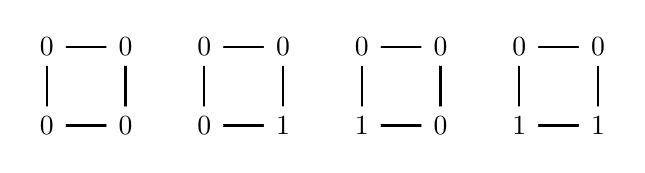
\begin{tikzpicture}
        % row1
        \cell{0}{0}{1}{1}
        \cell{2}{0}{3}{1}
        \cell{4}{0}{5}{1}
        \cell{6}{0}{7}{1}

        \( \lablvertex{0}{0}{$0$} \)
        \( \lablvertex{1}{0}{$0$} \)
        \( \lablvertex{2}{0}{$0$} \)
        \( \lablvertex{3}{0}{$1$} \)
        \( \lablvertex{4}{0}{$1$} \)
        \( \lablvertex{5}{0}{$0$} \)
        \( \lablvertex{6}{0}{$1$} \)
        \( \lablvertex{7}{0}{$1$} \)

        \( \lablvertex{0}{1}{$0$} \)
        \( \lablvertex{1}{1}{$0$} \)
        \( \lablvertex{2}{1}{$0$} \)
        \( \lablvertex{3}{1}{$0$} \)
        \( \lablvertex{4}{1}{$0$} \)
        \( \lablvertex{5}{1}{$0$} \)
        \( \lablvertex{6}{1}{$0$} \)
        \( \lablvertex{7}{1}{$0$} \)
        
    \end{tikzpicture}
\end{center}

For example, for the $m=2$ column with index $(0,1)$, this operation looks like the following.

\begin{center}
    \begin{tikzpicture}
        % row1
        \cell{-4.5}{2.5}{-3.5}{3.5}
        \cell{-4.5}{3.5}{-3.5}{4.5}

        % row 1
        \( \lablvertex{-4.5}{2.5}{$0$} \)
        \( \lablvertex{-4.5}{3.5}{$0$} \)
        \( \lablvertex{-4.5}{4.5}{$0$} \)
        
        \( \lablvertex{-3.5}{2.5}{$0$} \)
        \( \lablvertex{-3.5}{3.5}{$1$} \)
        \( \lablvertex{-3.5}{4.5}{$0$} \)

        % label
        \( \lablnode{-4}{1.5}{$A(2)_{0,1}$} \)

        % arrow
        \( \lablnode{-2}{3.5}{$\pmb{\to}$} \)

        % four columns
        \cell{0}{0}{1}{1}
        \cell{0}{1}{1}{2}
        \cell{0}{2}{1}{3}

        \cell{2}{0}{3}{1}
        \cell{2}{1}{3}{2}
        \cell{2}{2}{3}{3}

        \( \lablvertex{0}{0}{$0$} \)
        \( \lablvertex{0}{1}{$0$} \)
        \( \lablvertex{0}{2}{$1$} \)
        \( \lablvertex{0}{3}{$0$} \)
        
        \( \lablvertex{1}{0}{$0$} \)
        \( \lablvertex{1}{1}{$1$} \)
        \( \lablvertex{1}{2}{$0$} \)
        \( \lablvertex{1}{3}{$0$} \)
        
        \( \lablvertex{2}{0}{$0$} \)
        \( \lablvertex{2}{1}{$0$} \)
        \( \lablvertex{2}{2}{$1$} \)
        \( \lablvertex{2}{3}{$0$} \)
        
        \( \lablvertex{3}{0}{$0$} \)
        \( \lablvertex{3}{1}{$1$} \)
        \( \lablvertex{3}{2}{$1$} \)
        \( \lablvertex{3}{3}{$0$} \)
        
        \cell{0}{4}{1}{5}
        \cell{0}{5}{1}{6}
        \cell{0}{6}{1}{7}
        
        \cell{2}{4}{3}{5}
        \cell{2}{5}{3}{6}
        \cell{2}{6}{3}{7}

        \( \lablvertex{0}{4}{$0$} \)
        \( \lablvertex{0}{5}{$0$} \)
        \( \lablvertex{0}{6}{$0$} \)
        \( \lablvertex{0}{7}{$0$} \)
        
        \( \lablvertex{1}{4}{$0$} \)
        \( \lablvertex{1}{5}{$1$} \)
        \( \lablvertex{1}{6}{$0$} \)
        \( \lablvertex{1}{7}{$0$} \)
        
        \( \lablvertex{2}{4}{$0$} \)
        \( \lablvertex{2}{5}{$0$} \)
        \( \lablvertex{2}{6}{$0$} \)
        \( \lablvertex{2}{7}{$0$} \)
        
        \( \lablvertex{3}{4}{$0$} \)
        \( \lablvertex{3}{5}{$1$} \)
        \( \lablvertex{3}{6}{$1$} \)
        \( \lablvertex{3}{7}{$0$} \)

        \( \lablnode{5}{3.5}{$\pmb{\to}$} \)

        \( \lablnode{7.5}{3.5}{$\begin{bmatrix} A(3)_{0,2} & A(3)_{0,3} \\ A(3)_{1,2} & A(3)_{1,3} \end{bmatrix}$} \)

    \end{tikzpicture}
\end{center}

This operation results in $4$ new columns that are represented in $A(k+1)$. In our example, specifically we get the following. 

$$
\begin{bmatrix} 
    A(3)_{0,2} & A(3)_{0,3} \\ 
    A(3)_{1,2} & A(3)_{1,3} 
\end{bmatrix} = 
\begin{bmatrix} 
    1A(2)_{i,j} & 1A(2)_{i,j} \\ 
    0A(2)_{i,j} & 1A(2)_{i,j} 
\end{bmatrix},
$$

Critically, this transformation \textit{only} changes the identity of the top two tiles. This implies that the same value coefficients computed by comparing $A(2)$ and $A(3)$ can be used for any $m \times 1$ column, as long as both column indices $(i,j)$ are congruent $\text{mod } 2$. Furthermore, if one writes $A(k)$ as the block matrix

$$A(k) = \begin{bmatrix} A_{0,0} & A_{0,1} \\ A_{1,0} & A_{1,1} \end{bmatrix},$$

where $A_{\hat{i},\hat{j}} \in \mathbb{R}^{2^{k-2} \times 2^{k-2}}$, then all column's represented in $A_{\hat{i},\hat{j}}$ have indices $(i,j) \equiv (\hat{i},\hat{j}) \text{ mod } 2$. This allows us to write that in general, if $A(k) = \begin{bmatrix} A_{0,0} & A_{0,1} \\ A_{1,0} & A_{1,1} \end{bmatrix},$
then
$$A(k+1) = 
\begin{bmatrix}
    V_{0,0}A_{0,0} & V_{0,1}A_{0,0} & V_{0,2}A_{0,1} & V_{0,3}A_{0,1} \\
    V_{1,0}A_{0,0} & V_{1,1}A_{0,0} & V_{1,2}A_{0,1} & V_{1,3}A_{0,1} \\
    V_{2,0}A_{1,0} & V_{2,1}A_{1,0} & V_{2,2}A_{1,1} & V_{2,3}A_{1,1} \\
    V_{3,0}A_{1,0} & V_{3,1}A_{1,0} & V_{3,2}A_{1,1} & V_{3,3}A_{1,1} \\
\end{bmatrix}.
$$

where $V \in \mathbb{R}^{4 \times 4}$ can be found after directly computing $A(2)$ and $A(3)$, then solving the following equation.

$$
\begin{bmatrix}
    A(3)_{0,0} & A(3)_{0,1} & A(3)_{0,2} & A(3)_{0,3} \\
    A(3)_{1,0} & A(3)_{1,1} & A(3)_{1,2} & A(3)_{1,3} \\
    A(3)_{2,0} & A(3)_{2,1} & A(3)_{2,2} & A(3)_{2,3} \\
    A(3)_{3,0} & A(3)_{3,1} & A(3)_{3,2} & A(3)_{3,3} \\
\end{bmatrix} = 
\begin{bmatrix}
    V_{0,0}A(2)_{0,0} & V_{0,1}A(2)_{0,0} & V_{0,2}A(2)_{0,1} & V_{0,3}A(2)_{0,1} \\
    V_{1,0}A(2)_{0,0} & V_{1,1}A(2)_{0,0} & V_{1,2}A(2)_{0,1} & V_{1,3}A(2)_{0,1} \\
    V_{2,0}A(2)_{1,0} & V_{2,1}A(2)_{1,0} & V_{2,2}A(2)_{1,1} & V_{2,3}A(2)_{1,1} \\
    V_{3,0}A(2)_{1,0} & V_{3,1}A(2)_{1,0} & V_{3,2}A(2)_{1,1} & V_{3,3}A(2)_{1,1} \\
\end{bmatrix}
$$

This is easily solved to give 

$$V = 
\begin{bmatrix} 
    1 & 1 & 1 & 1 \\ 
    1 & 1 & 0 & 1 \\ 
    1 & 0 & 1 & 1 \\ 
    1 & 1 & 1 & 1 
\end{bmatrix}
$$


which completes the proof.

\end{proof}

The method detailed in Theorem \ref{thm: main theorem} generalizes to other tile sets, which we tabularize in Section \ref{section: summary of results} without proof. Interestingly, the method not only generalizes to other tile sets, but can also be augmented to enumerate the more complicated ``messy" polygon mosaics.

\section{Messy Polygon Mosaics}

A \textit{messy polygon mosaic} is a mosaic that contains at least one polygon, with no restriction on other shared edges. 

\begin{exmp}
\label{exmp: messy sap}
Below is a messy polygon mosaic of size $(5,7)$ that contains $1$ polygon, with the squares that make it up hilighted in gray. 

\begin{center}
    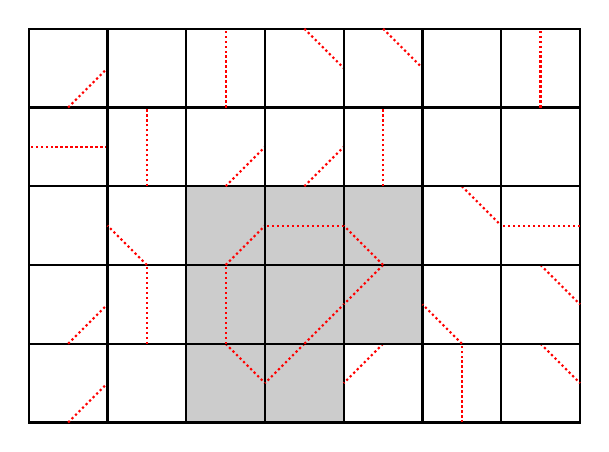
\begin{tikzpicture}
        % row1
        \cellA{0}{0}{1}{1}
        \cell{1}{0}{2}{1}
        \cellDf{2}{0}{3}{1}
        \cellCf{3}{0}{4}{1}
        \cellC{4}{0}{5}{1}
        \cellE{5}{0}{6}{1}
        \cellD{6}{0}{7}{1}
        % row2
        \cellA{0}{1}{1}{2}
        \cellE{1}{1}{2}{2}
        \cellEf{2}{1}{3}{2}
        \cellAf{3}{1}{4}{2}
        \cellCf{4}{1}{5}{2}
        \cellB{5}{1}{6}{2}
        \cellD{6}{1}{7}{2}
        % row3
        \cell{0}{2}{1}{3}
        \cellB{1}{2}{2}{3}
        \cellAf{2}{2}{3}{3}
        \cellFf{3}{2}{4}{3}
        \cellBf{4}{2}{5}{3}
        \cellD{5}{2}{6}{3}
        \cellF{6}{2}{7}{3}
        % row4
        \cellF{0}{3}{1}{4}
        \cellE{1}{3}{2}{4}
        \cellA{2}{3}{3}{4}
        \cellA{3}{3}{4}{4}
        \cellE{4}{3}{5}{4}
        \cell{5}{3}{6}{4}
        \cell{6}{3}{7}{4}
        % row5
        \cellA{0}{4}{1}{5}
        \cell{1}{4}{2}{5}
        \cellE{2}{4}{3}{5}
        \cellD{3}{4}{4}{5}
        \cellD{4}{4}{5}{5}
        \cell{5}{4}{6}{5}
        \cellE{6}{4}{7}{5}
    \end{tikzpicture}
\end{center}
\end{exmp}

It turns out that it is easier to enumerate the number of messy mosaics that \textit{do not} contain a polygon. Therefore, let $t_{m,n}$ be the number of mosaics that do not contain a polygon. Also from the fact that the smallest polygon is

\begin{center}
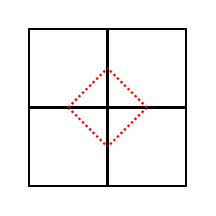
\begin{tikzpicture}
    % row1
    \cellD{0}{0}{1}{1}
    \cellC{1}{0}{2}{1}
    % row2
    \cellA{0}{1}{1}{2}
    \cellB{1}{1}{2}{2}
\end{tikzpicture}
\end{center}

we have that $t_{n,1}=7^n$, and $t_{2,2} = 7^4 - 1$. It turns out that using similar techniques to Theorem \ref{thm: main theorem} we can exactly enumerate messy mosaics. We define $A(m) \in \mathbb{Z}^{2^{m-1} \times 2^{m-1}}$, which we use to enumerate $t_{m,n}$.

\begin{defn}

First define $A(2) = \begin{bmatrix}
7^2 & 1 \\
-1 & 1
\end{bmatrix}$. 

We recursively define $A(k+1) \in \mathbb{Z}^{2^{n-1} \times 2^{n-1}}$ given $A(k)$. Begin by writing
$
A(k) = \begin{bmatrix}
A_{0,0} & A_{0,1} \\
A_{1,0} & A_{1,1}
\end{bmatrix}
$, where the block matrices $A_{i,j}$ are square block matrices of size $2^{k-2} \times 2^{k-2}$. We then have

$$
A(k+1) = \begin{bmatrix}
    7A_{0,0} & \frac{1}{7}A_{0,0} & 7A_{0,1} & A_{0,1} \\
    -\frac{1}{7}A_{0,0} & \frac{1}{7}A_{0,0} & 0A_{0,1} & A_{0,1} \\
    7A_{1,0} & 0A_{1,0} & 7A_{1,1}  & A_{1,1} \\
    A_{1,0} & -A_{1,0} & -A_{1,1} & 7A_{1,1} \\
\end{bmatrix}.
$$

Construct $A(m)$ by starting with $k=2$ and recursing until $k=m$. 

\end{defn}

\begin{thm}
\label{thm: messy mosaics}
The number of messy mosaics that \textit{do not} contain a polygon is the $(0,0)$-th entry of $A(m)^n$.
\end{thm}

\section{Proof of Theorem \ref{thm: messy mosaics}}

\begin{proof}
We consider the same vertex labeling in the proof of Theorem \ref{thm: main theorem}, namely labeling a vertex by the number of polygons that contain it $\text{mod } 2$. However, there is not a bijection between messy polygon mosaics and vertex labelings as there is with polygon mosaics. This is because the following cell-labellings configurations are no longer uniquely determined.

\begin{center}
    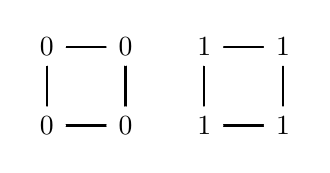
\begin{tikzpicture}
        % row1
        \cell{0}{0}{1}{1}
        \cell{2}{0}{3}{1}

        \( \lablvertex{0}{0}{$0$} \)
        \( \lablvertex{1}{0}{$0$} \)
        \( \lablvertex{2}{0}{$1$} \)
        \( \lablvertex{3}{0}{$1$} \)

        \( \lablvertex{0}{1}{$0$} \)
        \( \lablvertex{1}{1}{$0$} \)
        \( \lablvertex{2}{1}{$1$} \)
        \( \lablvertex{3}{1}{$1$} \)
    \end{tikzpicture}
\end{center}

Additionally, the sub-grid vertex labelings shown below

\begin{center}
    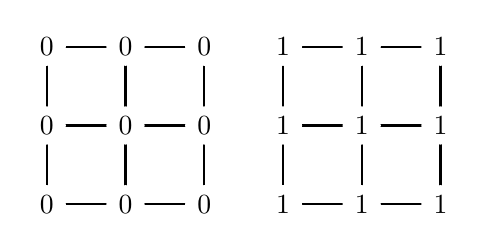
\begin{tikzpicture}
        % row1
        \cell{0}{0}{1}{1}
        \cell{0}{1}{1}{2}
        \cell{1}{0}{2}{1}
        \cell{1}{1}{2}{2}

        \( \lablvertex{0}{0}{$0$} \)
        \( \lablvertex{1}{0}{$0$} \)
        \( \lablvertex{2}{0}{$0$} \)

        \( \lablvertex{0}{1}{$0$} \)
        \( \lablvertex{1}{1}{$0$} \)
        \( \lablvertex{2}{1}{$0$} \)
        
        \( \lablvertex{0}{2}{$0$} \)
        \( \lablvertex{1}{2}{$0$} \)
        \( \lablvertex{2}{2}{$0$} \)
        
        % row1
        \cell{3}{0}{4}{1}
        \cell{3}{1}{4}{2}
        \cell{4}{0}{5}{1}
        \cell{4}{1}{5}{2}

        \( \lablvertex{3}{0}{$1$} \)
        \( \lablvertex{4}{0}{$1$} \)
        \( \lablvertex{5}{0}{$1$} \)

        \( \lablvertex{3}{1}{$1$} \)
        \( \lablvertex{4}{1}{$1$} \)
        \( \lablvertex{5}{1}{$1$} \)

        \( \lablvertex{3}{2}{$1$} \)
        \( \lablvertex{4}{2}{$1$} \)
        \( \lablvertex{5}{2}{$1$} \)

    \end{tikzpicture}
\end{center}

are now ambiguous as to whether or not they represent a polygon. For example, both of the following vertex labelings could include the right-most messy polygon mosaic. 

\begin{center}
    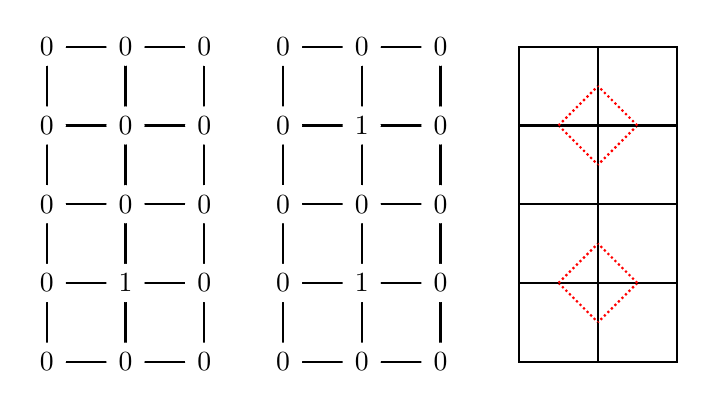
\begin{tikzpicture}
        % row1
        \cell{0}{0}{1}{1}
        \cell{0}{1}{1}{2}
        \cell{0}{2}{1}{3}
        \cell{0}{3}{1}{4}
        \cell{1}{0}{2}{1}
        \cell{1}{1}{2}{2}
        \cell{1}{2}{2}{3}
        \cell{1}{3}{2}{4}
        
        \( \lablvertex{0}{0}{$0$} \)
        \( \lablvertex{1}{0}{$0$} \)
        \( \lablvertex{2}{0}{$0$} \)

        \( \lablvertex{0}{1}{$0$} \)
        \( \lablvertex{1}{1}{$1$} \)
        \( \lablvertex{2}{1}{$0$} \)

        \( \lablvertex{0}{2}{$0$} \)
        \( \lablvertex{1}{2}{$0$} \)
        \( \lablvertex{2}{2}{$0$} \)

        \( \lablvertex{0}{3}{$0$} \)
        \( \lablvertex{1}{3}{$0$} \)
        \( \lablvertex{2}{3}{$0$} \)

        \( \lablvertex{0}{4}{$0$} \)
        \( \lablvertex{1}{4}{$0$} \)
        \( \lablvertex{2}{4}{$0$} \)

        % row1
        \cell{3}{0}{4}{1}
        \cell{3}{1}{4}{2}
        \cell{3}{2}{4}{3}
        \cell{3}{3}{4}{4}
        \cell{4}{0}{5}{1}
        \cell{4}{1}{5}{2}
        \cell{4}{2}{5}{3}
        \cell{4}{3}{5}{4}

        \( \lablvertex{3}{0}{$0$} \)
        \( \lablvertex{4}{0}{$0$} \)
        \( \lablvertex{5}{0}{$0$} \)

        \( \lablvertex{3}{1}{$0$} \)
        \( \lablvertex{4}{1}{$1$} \)
        \( \lablvertex{5}{1}{$0$} \)

        \( \lablvertex{3}{2}{$0$} \)
        \( \lablvertex{4}{2}{$0$} \)
        \( \lablvertex{5}{2}{$0$} \)

        \( \lablvertex{3}{3}{$0$} \)
        \( \lablvertex{4}{3}{$1$} \)
        \( \lablvertex{5}{3}{$0$} \)

        \( \lablvertex{3}{4}{$0$} \)
        \( \lablvertex{4}{4}{$0$} \)
        \( \lablvertex{5}{4}{$0$} \)

        \cellD{6}{0}{7}{1}
        \cellC{7}{0}{8}{1}

        \cellA{6}{1}{7}{2}
        \cellB{7}{1}{8}{2}

        \cellD{6}{2}{7}{3}
        \cellC{7}{2}{8}{3}    

        \cellA{6}{3}{7}{4}
        \cellB{7}{3}{8}{4}    

    \end{tikzpicture}
\end{center}

Critically, the number of polygons that appear in a given messy polygon mosaic is exactly the number of parity configurations that map to that mosaic. 
Therefore, if we are to count these mosaics, we need to account for this double-counting with the inclusion-exclusion principle.  

To create an analagous result to Theorem \ref{thm: main theorem} we need to find a weight assignment to the $16$ parity configurations below that fulfill a set of conditions.

\begin{center}
    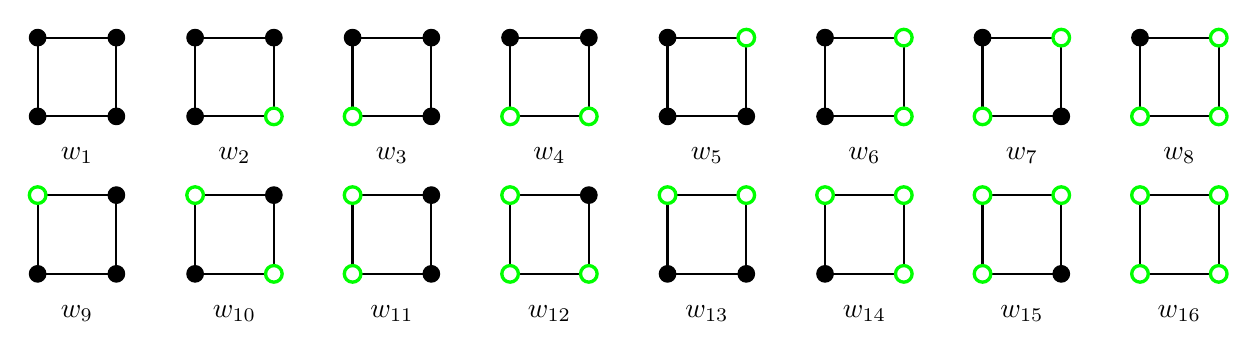
\begin{tikzpicture}
        % row1
        \cell{0}{0}{1}{1}
        \cell{2}{0}{3}{1}
        \cell{4}{0}{5}{1}
        \cell{6}{0}{7}{1}
        \cell{8}{0}{9}{1}
        \cell{10}{0}{11}{1}
        \cell{12}{0}{13}{1}
        \cell{14}{0}{15}{1}
        % row2
        \cell{0}{2}{1}{3}
        \cell{2}{2}{3}{3}This means that
        \cell{4}{2}{5}{3}
        \cell{6}{2}{7}{3}
        \cell{8}{2}{9}{3}
        \cell{10}{2}{11}{3}
        \cell{12}{2}{13}{3}
        \cell{14}{2}{15}{3}
        % label for row1
        \draw[fill=black] (0,0) circle (3pt);
        \draw[fill=black] (1,0) circle (3pt);
        \draw[fill=black] (2,0) circle (3pt);
        \draw[fill=white, draw=green, very thick] (3,0) circle (3pt);
        \draw[fill=white, draw=green, very thick] (4,0) circle (3pt);
        \draw[fill=black] (5,0) circle (3pt);
        \draw[fill=white, draw=green, very thick] (6,0) circle (3pt);
        \draw[fill=white, draw=green, very thick] (7,0) circle (3pt);
        \draw[fill=black] (8,0) circle (3pt);
        \draw[fill=black] (9,0) circle (3pt);
        \draw[fill=black] (10,0) circle (3pt);
        \draw[fill=white, draw=green, very thick] (11,0) circle (3pt);
        \draw[fill=white, draw=green, very thick] (12,0) circle (3pt);
        \draw[fill=black] (13,0) circle (3pt);
        \draw[fill=white, draw=green, very thick] (14,0) circle (3pt);
        \draw[fill=white, draw=green, very thick] (15,0) circle (3pt);
        % label for row1
        \draw[fill=white, draw=green, very thick] (0,1) circle (3pt);
        \draw[fill=black] (1,1) circle (3pt);
        \draw[fill=white, draw=green, very thick] (2,1) circle (3pt);
        \draw[fill=black] (3,1) circle (3pt);
        \draw[fill=white, draw=green, very thick] (4,1) circle (3pt);
        \draw[fill=black] (5,1) circle (3pt);
        \draw[fill=white, draw=green, very thick] (6,1) circle (3pt);
        \draw[fill=black] (7,1) circle (3pt);
        \draw[fill=white, draw=green, very thick] (8,1) circle (3pt);
        \draw[fill=white, draw=green, very thick] (9,1) circle (3pt);
        \draw[fill=white, draw=green, very thick] (10,1) circle (3pt);
        \draw[fill=white, draw=green, very thick] (11,1) circle (3pt);
        \draw[fill=white, draw=green, very thick] (12,1) circle (3pt);
        \draw[fill=white, draw=green, very thick] (13,1) circle (3pt);
        \draw[fill=white, draw=green, very thick] (14,1) circle (3pt);
        \draw[fill=white, draw=green, very thick] (15,1) circle (3pt);
        % label for row1
        \draw[fill=black] (0,2) circle (3pt);
        \draw[fill=black] (1,2) circle (3pt);
        \draw[fill=black] (2,2) circle (3pt);
        \draw[fill=white, draw=green, very thick] (3,2) circle (3pt);
        \draw[fill=white, draw=green, very thick] (4,2) circle (3pt);
        \draw[fill=black] (5,2) circle (3pt);
        \draw[fill=white, draw=green, very thick] (6,2) circle (3pt);
        \draw[fill=white, draw=green, very thick] (7,2) circle (3pt);
        \draw[fill=black] (8,2) circle (3pt);
        \draw[fill=black] (9,2) circle (3pt);
        \draw[fill=black] (10,2) circle (3pt);
        \draw[fill=white, draw=green, very thick] (11,2) circle (3pt);
        \draw[fill=white, draw=green, very thick] (12,2) circle (3pt);
        \draw[fill=black] (13,2) circle (3pt);
        \draw[fill=white, draw=green, very thick] (14,2) circle (3pt);
        \draw[fill=white, draw=green, very thick] (15,2) circle (3pt);
        % label for row1
        \draw[fill=black] (0,3) circle (3pt);
        \draw[fill=black] (1,3) circle (3pt);
        \draw[fill=black] (2,3) circle (3pt);
        \draw[fill=black] (3,3) circle (3pt);
        \draw[fill=black] (4,3) circle (3pt);
        \draw[fill=black] (5,3) circle (3pt);
        \draw[fill=black] (6,3) circle (3pt);
        \draw[fill=black] (7,3) circle (3pt);
        \draw[fill=black] (8,3) circle (3pt);
        \draw[fill=white, draw=green, very thick] (9,3) circle (3pt);
        \draw[fill=black] (10,3) circle (3pt);
        \draw[fill=white, draw=green, very thick] (11,3) circle (3pt);
        \draw[fill=black] (12,3) circle (3pt);
        \draw[fill=white, draw=green, very thick] (13,3) circle (3pt);
        \draw[fill=black] (14,3) circle (3pt);
        \draw[fill=white, draw=green, very thick] (15,3) circle (3pt);
        % numbers row 1
        \( \lablnode{0.5}{-0.5}{$w_{9}$} \)
        \( \lablnode{2.5}{-0.5}{$w_{10}$} \)
        \( \lablnode{4.5}{-0.5}{$w_{11}$} \)
        \( \lablnode{6.5}{-0.5}{$w_{12}$} \)
        \( \lablnode{8.5}{-0.5}{$w_{13}$} \)
        \( \lablnode{10.5}{-0.5}{$w_{14}$} \)
        \( \lablnode{12.5}{-0.5}{$w_{15}$} \)
        \( \lablnode{14.5}{-0.5}{$w_{16}$} \)
        % numbers row 2
        \( \lablnode{0.5}{1.5}{$w_{1}$} \)
        \( \lablnode{2.5}{1.5}{$w_{2}$} \)
        \( \lablnode{4.5}{1.5}{$w_{3}$} \)
        \( \lablnode{6.5}{1.5}{$w_{4}$} \)
        \( \lablnode{8.5}{1.5}{$w_{5}$} \)
        \( \lablnode{10.5}{1.5}{$w_{6}$} \)
        \( \lablnode{12.5}{1.5}{$w_{7}$} \)
        \( \lablnode{14.5}{1.5}{$w_{8}$} \)
    \end{tikzpicture}
\end{center}

First $w_{7}=w_{10}=0$, as again these are impossible parity configurations for our tile set. Next notice that $w_{1} = w_{16} = b$, as these cells do not indicate a specific tile.  The remaining weights uniquely specify a tile, and so are equal to $1$ or $-1$. But how do we find these assignments?

First notice that we want a weight assignment so that the parity configurations for a given polygon multiply to $-1$. This is due to the inclusion-exclusion principle. This means that if there are multiple polygons in a mosaic, then the product will be positive if there is an even number of polygons specified, and negative if there is an odd number specified.

Next note the following lemma.
\begin{lemma}
    \label{lemma: build bigger saps}
    One can construct all larger polygons from the smallest polygon using a finite set of transformations $S$.
\end{lemma}

\begin{proof}
    TODO
\end{proof}

This is because one can find $w_{1} , \dots, w_{16}$ so that the following two constraints hold:

\begin{constraint}
    \label{constraint: smallest sap prod}
    The weights associated with the smallest polygon multiply to $-1$, ie. $w_2 w_3 w_5 w_9 = -1.$ 
\end{constraint}

\begin{constraint}
    \label{constraint: prod works}
    \emph{All} transformations in $S$ preserve the weight product of a changed polygon.
\end{constraint}

Constraint \ref{constraint: smallest sap prod} and Constraint \ref{constraint: prod works} amount to a series of constraints on the values of $w_i$. The derivation for these constraints can be found in the Appendix. Choosing a solution set from these constraints gives the following weights.

\begin{center}
    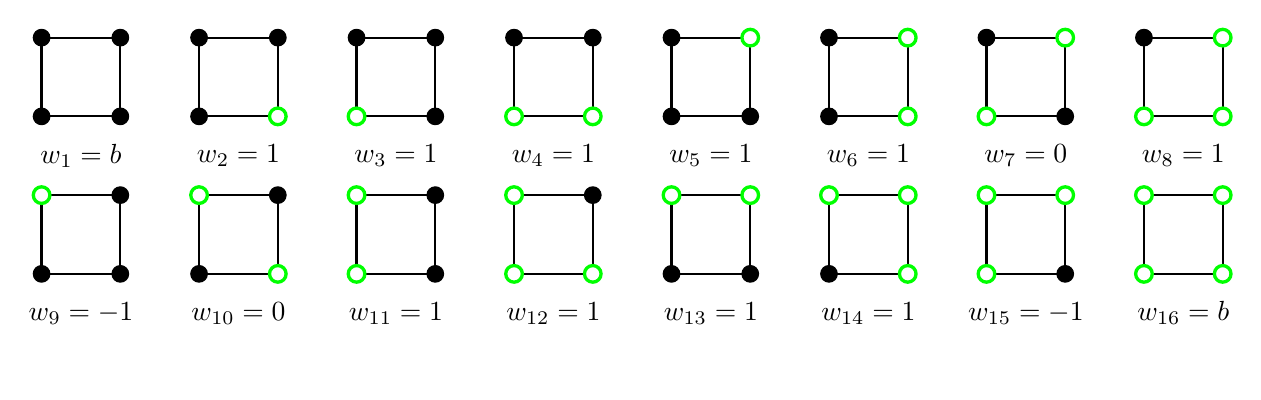
\begin{tikzpicture}
        % row1
        \cell{0}{0}{1}{1}
        \cell{2}{0}{3}{1}
        \cell{4}{0}{5}{1}
        \cell{6}{0}{7}{1}
        \cell{8}{0}{9}{1}
        \cell{10}{0}{11}{1}
        \cell{12}{0}{13}{1}
        \cell{14}{0}{15}{1}
        % row2
        \cell{0}{2}{1}{3}
        \cell{2}{2}{3}{3}
        \cell{4}{2}{5}{3}
        \cell{6}{2}{7}{3}
        \cell{8}{2}{9}{3}
        \cell{10}{2}{11}{3}
        \cell{12}{2}{13}{3}
        \cell{14}{2}{15}{3}
        % label for row1
        \draw[fill=black] (0,0) circle (3pt);
        \draw[fill=black] (1,0) circle (3pt);
        \draw[fill=black] (2,0) circle (3pt);
        \draw[fill=white, draw=green, very thick] (3,0) circle (3pt);
        \draw[fill=white, draw=green, very thick] (4,0) circle (3pt);
        \draw[fill=black] (5,0) circle (3pt);
        \draw[fill=white, draw=green, very thick] (6,0) circle (3pt);
        \draw[fill=white, draw=green, very thick] (7,0) circle (3pt);
        \draw[fill=black] (8,0) circle (3pt);
        \draw[fill=black] (9,0) circle (3pt);
        \draw[fill=black] (10,0) circle (3pt);
        \draw[fill=white, draw=green, very thick] (11,0) circle (3pt);
        \draw[fill=white, draw=green, very thick] (12,0) circle (3pt);
        \draw[fill=black] (13,0) circle (3pt);
        \draw[fill=white, draw=green, very thick] (14,0) circle (3pt);
        \draw[fill=white, draw=green, very thick] (15,0) circle (3pt);
        % label for row1
        \draw[fill=white, draw=green, very thick] (0,1) circle (3pt);
        \draw[fill=black] (1,1) circle (3pt);
        \draw[fill=white, draw=green, very thick] (2,1) circle (3pt);
        \draw[fill=black] (3,1) circle (3pt);
        \draw[fill=white, draw=green, very thick] (4,1) circle (3pt);
        \draw[fill=black] (5,1) circle (3pt);
        \draw[fill=white, draw=green, very thick] (6,1) circle (3pt);
        \draw[fill=black] (7,1) circle (3pt);
        \draw[fill=white, draw=green, very thick] (8,1) circle (3pt);
        \draw[fill=white, draw=green, very thick] (9,1) circle (3pt);
        \draw[fill=white, draw=green, very thick] (10,1) circle (3pt);
        \draw[fill=white, draw=green, very thick] (11,1) circle (3pt);
        \draw[fill=white, draw=green, very thick] (12,1) circle (3pt);
        \draw[fill=white, draw=green, very thick] (13,1) circle (3pt);
        \draw[fill=white, draw=green, very thick] (14,1) circle (3pt);
        \draw[fill=white, draw=green, very thick] (15,1) circle (3pt);
        % label for row1
        \draw[fill=black] (0,2) circle (3pt);
        \draw[fill=black] (1,2) circle (3pt);
        \draw[fill=black] (2,2) circle (3pt);
        \draw[fill=white, draw=green, very thick] (3,2) circle (3pt);
        \draw[fill=white, draw=green, very thick] (4,2) circle (3pt);
        \draw[fill=black] (5,2) circle (3pt);
        \draw[fill=white, draw=green, very thick] (6,2) circle (3pt);
        \draw[fill=white, draw=green, very thick] (7,2) circle (3pt);
        \draw[fill=black] (8,2) circle (3pt);
        \draw[fill=black] (9,2) circle (3pt);
        \draw[fill=black] (10,2) circle (3pt);
        \draw[fill=white, draw=green, very thick] (11,2) circle (3pt);
        \draw[fill=white, draw=green, very thick] (12,2) circle (3pt);
        \draw[fill=black] (13,2) circle (3pt);
        \draw[fill=white, draw=green, very thick] (14,2) circle (3pt);
        \draw[fill=white, draw=green, very thick] (15,2) circle (3pt);
        % label for row1
        \draw[fill=black] (0,3) circle (3pt);
        \draw[fill=black] (1,3) circle (3pt);
        \draw[fill=black] (2,3) circle (3pt);
        \draw[fill=black] (3,3) circle (3pt);
        \draw[fill=black] (4,3) circle (3pt);
        \draw[fill=black] (5,3) circle (3pt);
        \draw[fill=black] (6,3) circle (3pt);
        \draw[fill=black] (7,3) circle (3pt);
        \draw[fill=black] (8,3) circle (3pt);
        \draw[fill=white, draw=green, very thick] (9,3) circle (3pt);
        \draw[fill=black] (10,3) circle (3pt);
        \draw[fill=white, draw=green, very thick] (11,3) circle (3pt);
        \draw[fill=black] (12,3) circle (3pt);
        \draw[fill=white, draw=green, very thick] (13,3) circle (3pt);
        \draw[fill=black] (14,3) circle (3pt);
        \draw[fill=white, draw=green, very thick] (15,3) circle (3pt);
        % numbers row 1
        \( \lablnode{0.5}{-0.5}{$w_{9}=-1$} \)
        \( \lablnode{2.5}{-0.5}{$w_{10}=0$} \)
        \( \lablnode{4.5}{-0.5}{$w_{11}=1$} \)
        \( \lablnode{6.5}{-0.5}{$w_{12}=1$} \)
        \( \lablnode{8.5}{-0.5}{$w_{13}=1$} \)
        \( \lablnode{10.5}{-0.5}{$w_{14}=1$} \)
        \( \lablnode{12.5}{-0.5}{$w_{15}=-1$} \)
        \( \lablnode{14.5}{-0.5}{$w_{16}=b$} \)
        % numbers row 2
        \( \lablnode{0.5}{1.5}{$w_{1}=b$} \)
        \( \lablnode{2.5}{1.5}{$w_{2}=1$} \)
        \( \lablnode{4.5}{1.5}{$w_{3}=1$} \)
        \( \lablnode{6.5}{1.5}{$w_{4}=1$} \)
        \( \lablnode{8.5}{1.5}{$w_{5}=1$} \)
        \( \lablnode{10.5}{1.5}{$w_{6}=1$} \)
        \( \lablnode{12.5}{1.5}{$w_{7}=0$} \)
        \( \lablnode{14.5}{1.5}{$w_{8}=1$} \)
    \end{tikzpicture}
\end{center}

This immediately gives us a way to construct an analagous definition for our transition matrixes $A(k) = \begin{bmatrix} A_1 & A_2 \\ A_3 & A_4 \end{bmatrix}$. As the appending of a cell parity configuration can possibly change the number of admitted cells, we define $v_{1} ,\dots, v_{16}$ for the associated change in the number of mosaics for the recursive definition of $A(k+1)$. A simple way to obtain $v_{1} ,\dots, v_{16}$ is to directly compute $A(2)$ and $A(3)$ and compare their values like so.

$$A(2) = 
\begin{bmatrix}
    b^2 & 1 \\
    -1 & 1
\end{bmatrix}, A(3)=
\begin{bmatrix}
b^3 & b & b & 1 \\
-b & b & 0 & 1 \\
-b & 0 & b & 1 \\
-1 & 1 & 1 & b \\
\end{bmatrix}.$$

This gives

$$
A(k+1) = 
\begin{bmatrix}
    v_{1}A_1 & v_{2}A_2 & v_{3}A_1 & v_{4}A_2 \\
    v_{5}A_3 & v_{6}A_4 & v_{7}A_3 & v_{8}A_4 \\
    v_{9}A_1 & v_{10}A_2 & v_{11}A_1 & v_{12}A_2 \\
    v_{13}A_3 & v_{14}A_4 & v_{15}A_3 & v_{16}A_4 \\
\end{bmatrix} =
\begin{bmatrix}
bA_1 & bA_2 & \frac{1}{b}A_1 & A_2 \\
bA_3 & bA_4 & 0A_3 & A_4 \\
-\frac{1}{b}A_1 & 0A_2 & \frac{1}{b}A_1 & A_2 \\
A_3 & A_4 & -A_3 & bA_4 \\
\end{bmatrix}.
$$

An analagous argument to Theorem \ref{thm: main theorem} then gives the result.

\end{proof}

% \begin{theorem}
%     \label{thm: growth rate}    
%     Let the probability that an $(m,n)$-mosaic \textit{does not} contain a SAP be denoted $p_{m,n} = \frac{t_{m,n}}{7^{nm}}$. Then the growth rate of the main diagonal $p_{n,n}$ has
%     $$\gamma = \lim_{n \to \infty} \frac{p_{n+1,n+1}p_{n-1,n-1}}{p_{n,n}^2} = ?$$
% \end{theorem}


\section{Summary of Results}
\label{section: summary of results}

Below is a tabulated summary of the results, where the matrices under the "Polygon Mosaics" and "Messy Polygon Mosaics" column are $A(2), W$. One can identify the number of  the number of (messy)

$$A(k+1) = W \cdot \begin{bmatrix}
    A_1(k) & A_2(k) \\
    A_3(k) & A_4(k)
    \end{bmatrix}$$

$$\begin{bmatrix}
    v_{1}A_1 & v_{2}A_2 & v_{3}A_1 & v_{4}A_2 \\
    v_{5}A_3 & v_{6}A_4 & v_{7}A_3 & v_{8}A_4 \\
    v_{9}A_1 & v_{10}A_2 & v_{11}A_1 & v_{12}A_2 \\
    v_{13}A_3 & v_{14}A_4 & v_{15}A_3 & v_{16}A_4 \\
\end{bmatrix}$$

Then the $(0,0)$-th entry of $A(m)^n$ is $p_{m,n}$ (polygon mosaics) and $t_{n,m}$ (mosaics that do not contain polygons).

TODO finish explan of following table

\begin{center}
    \begin{tblr}{
  colspec = {X[c,h]X[c]X[c]X[c]},
  stretch = 0,
  rowsep = 6pt,
  hlines = {black, 1pt},
  vlines = {black, 1pt},
}
  \textbf{Tile Set} & \textbf{Polygon Mosaics} & \textbf{Messy Polygon Mosaics}\\
  
  \resizebox{0.3\textwidth}{!}{%
  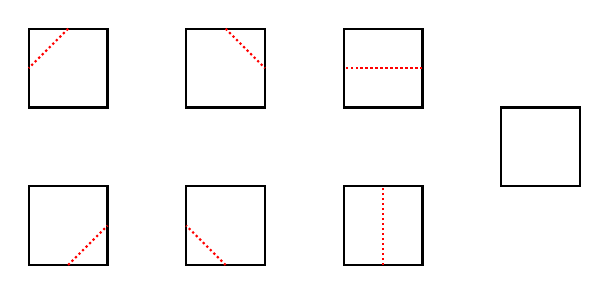
\begin{tikzpicture}
      \cellA{0}{0}{1}{1}
      \cellB{2}{0}{3}{1}
      \cellC{0}{2}{1}{3}
      \cellD{2}{2}{3}{3}
      
      \cellE{4}{0}{5}{1}
      \cellF{4}{2}{5}{3}

      \cell{6}{1}{7}{2}

    \end{tikzpicture}
    } 
    & 
    $\begin{bmatrix}
    1 & 1 \\
    1 & 1
    \end{bmatrix},
    \begin{bmatrix} 
    1 & 1 & 1 & 1 \\ 
    1 & 1 & 0 & 1 \\ 
    1 & 0 & 1 & 1 \\ 
    1 & 1 & 1 & 1 
    \end{bmatrix}$
    & 
    $\begin{bmatrix}
        7^2 & 1 \\
        -1 & 1
    \end{bmatrix},
    \begin{bmatrix} 
    7 & 7 & \frac{1}{7}& 1 \\ 
    7 & 7 & 0 & 1 \\ 
    -\frac{1}{7} & 0 & 1 & 1 \\ 
    1 & 1 & -1 & 7
    \end{bmatrix}$
    \\
    
    \resizebox{0.3\textwidth}{!}{%
    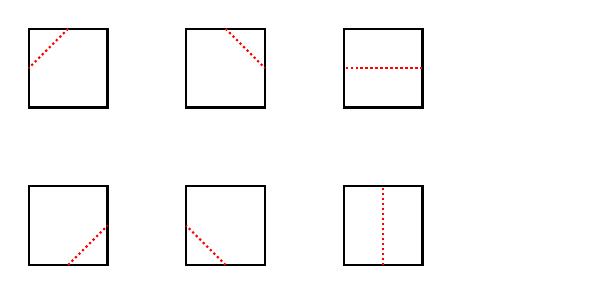
\begin{tikzpicture}
        \cellA{0}{0}{1}{1}
        \cellB{2}{0}{3}{1}
        \cellC{0}{2}{1}{3}
        \cellD{2}{2}{3}{3}
        
        \cellE{4}{0}{5}{1}
        \cellF{4}{2}{5}{3}
        % invisible cell for spacing
        \spacecell{6}{1}{7}{2}
    \end{tikzpicture}
    } 
    & 
    TODO 
    & 
    $\begin{bmatrix}
        6^2 & 1 \\
        -1 & 1
    \end{bmatrix},
    \begin{bmatrix} 
    6 & 6 & \frac{1}{6}& 1 \\ 
    6 & 6 & 0 & 1 \\ 
    -\frac{1}{6} & 0 & 1 & 1 \\ 
    1 & 1 & -1 & 6
    \end{bmatrix}$ 
    \\

    \resizebox{0.3\textwidth}{!}{%
    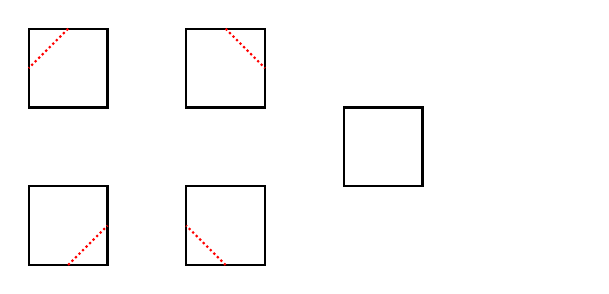
\begin{tikzpicture}
        \cellA{0}{0}{1}{1}
        \cellB{2}{0}{3}{1}
        \cellC{0}{2}{1}{3}
        \cellD{2}{2}{3}{3}
        
        \cell{4}{1}{5}{2}
        % invisible cell for spacing
        \spacecell{6}{1}{7}{2}
        
    \end{tikzpicture}
    } 
    & 
    $\begin{bmatrix}
        1 & 1 \\
        1 & 0
    \end{bmatrix}$, TODO 
    & 
    TODO
    \\

    \resizebox{0.3\textwidth}{!}{%
    \begin{tikzpicture}
        \cellA{0}{0}{1}{1}
        \cellB{2}{0}{3}{1}
        \cellC{0}{2}{1}{3}
        \cellD{2}{2}{3}{3}
        % invisible cell for spacing
        \spacecell{4}{1}{5}{2}
        % invisible cell for spacing
        \spacecell{6}{1}{7}{2}
    \end{tikzpicture}
      } 
    & 
    TODO
    & 
    TODO 
    \\
  
\end{tblr}
\end{center}


\printbibliography


\section{Appendix}

Flipping the parity of a single vertex in a parity configuration changes the $4$ surrounding cells. This creates a constraint on a subset of $w_1 ,\dots, w_{16}.$ 

The flipping of parity of a single vertex can result in $2$ distinct types of constraints. Let a constraint of \textit{Type 1} be a parity flip that does not change the number of polygons in the parity configuration. For example, consider the following flip of the center vertex in the following portion of a parity configuration.

\begin{center}
    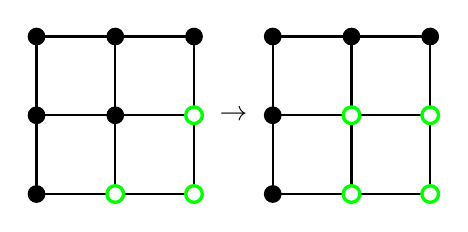
\begin{tikzpicture}
        % row1
        \cell{0}{0}{1}{1}
        \cell{1}{0}{2}{1}
        % row2
        \cell{0}{1}{1}{2}
        \cell{1}{1}{2}{2}
        % label for row1
        \draw[fill=black] (0,0) circle (3pt);
        \draw[fill=white, draw=green, very thick] (1,0) circle (3pt);
        \draw[fill=white, draw=green, very thick] (2,0) circle (3pt);
        % label for row2
        \draw[fill=black] (0,1) circle (3pt);
        \draw[fill=black] (1,1) circle (3pt);
        \draw[fill=white, draw=green, very thick] (2,1) circle (3pt);
        % label for row3
        \draw[fill=black] (0,2) circle (3pt);
        \draw[fill=black] (1,2) circle (3pt);
        \draw[fill=black] (2,2) circle (3pt);
        % row1
        \cell{3}{0}{4}{1}
        \cell{4}{0}{5}{1}
        % row2
        \cell{3}{1}{4}{2}
        \cell{4}{1}{5}{2}
        % label for row1
        \draw[fill=black] (3,0) circle (3pt);
        \draw[fill=white, draw=green, very thick] (4,0) circle (3pt);
        \draw[fill=white, draw=green, very thick] (5,0) circle (3pt);
        % label for row2
        \draw[fill=black] (3,1) circle (3pt);
        \draw[fill=white, draw=green, very thick] (4,1) circle (3pt);
        \draw[fill=white, draw=green, very thick] (5,1) circle (3pt);
        % label for row3
        \draw[fill=black] (3,2) circle (3pt);
        \draw[fill=black] (4,2) circle (3pt);
        \draw[fill=black] (5,2) circle (3pt);

        \( \lablnode{2.5}{1}{$\rightarrow$} \)
    \end{tikzpicture}
\end{center}

As this does not change the associated number of polygons in the larger parity configuration, we want this to preserve the sign of the weight product. This gives the following associated constraint. 

$$\text{sign}(w_{1}w_{2}w_{5}w_{9}) = \text{sign}(w_{2}w_{4}w_{6}w_{16}).$$

Now let a constraint of \textit{Type 2} be a parity flip that does change the number of polygons. For example, consider flipping the center vertex of the following portion of a parity configuration.

\begin{center}
    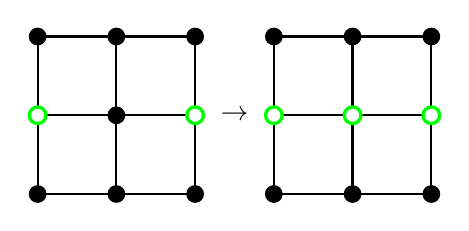
\begin{tikzpicture}
        % row1
        \cell{0}{0}{1}{1}
        \cell{1}{0}{2}{1}
        % row2
        \cell{0}{1}{1}{2}
        \cell{1}{1}{2}{2}
        % label for row1
        \draw[fill=black] (0,0) circle (3pt);
        \draw[fill=black] (1,0) circle (3pt);
        \draw[fill=black] (2,0) circle (3pt);
        % label for row2
        \draw[fill=white, draw=green, very thick] (0,1) circle (3pt);
        \draw[fill=black] (1,1) circle (3pt);
        \draw[fill=white, draw=green, very thick] (2,1) circle (3pt);
        % label for row3
        \draw[fill=black] (0,2) circle (3pt);
        \draw[fill=black] (1,2) circle (3pt);
        \draw[fill=black] (2,2) circle (3pt);
        % row1
        \cell{3}{0}{4}{1}
        \cell{4}{0}{5}{1}
        % row2
        \cell{3}{1}{4}{2}
        \cell{4}{1}{5}{2}
        % label for row1
        \draw[fill=black] (3,0) circle (3pt);
        \draw[fill=black] (4,0) circle (3pt);
        \draw[fill=black] (5,0) circle (3pt);
        % label for row2
        \draw[fill=white, draw=green, very thick] (3,1) circle (3pt);
        \draw[fill=white, draw=green, very thick] (4,1) circle (3pt);
        \draw[fill=white, draw=green, very thick] (5,1) circle (3pt);
        % label for row3
        \draw[fill=black] (3,2) circle (3pt);
        \draw[fill=black] (4,2) circle (3pt);
        \draw[fill=black] (5,2) circle (3pt);

        \( \lablnode{2.5}{1}{$\rightarrow$} \)
    \end{tikzpicture}
\end{center}

The above transformation corresponds with \textit{either} two distinct polygons joining into one polygon \textit{or} one polygon splitting into two distinct polygons. In either case, we want the sign of the product to switch. This corresponds with the following constraint.

$$\text{sign}(w_{3}w_{2}w_{9}w_{5}) = -\text{sign}(w_{4}w_{4}w_{13}w_{13}).$$

All Type 1 constraints are as follows. For the following set of equations, assume the equals sign ($=$) means \textit{only} equal in sign.

\begin{eqnarray*}
    w_{1}w_{1}w_{2}w_{3} = w_{2}w_{3}w_{6}w_{11} & w_{1}w_{1}w_{2}w_{4} = w_{2}w_{3}w_{6}w_{12} & w_{1}w_{1}w_{4}w_{3} = w_{2}w_{3}w_{8}w_{11} \\
    w_{1}w_{1}w_{4}w_{4} = w_{2}w_{3}w_{8}w_{12} & w_{1}w_{2}w_{1}w_{5} = w_{2}w_{4}w_{5}w_{13} & w_{1}w_{2}w_{1}w_{6} = w_{2}w_{4}w_{5}w_{14} \\
    w_{1}w_{2}w_{2}w_{8} = w_{2}w_{4}w_{6}w_{16} & w_{1}w_{2}w_{4}w_{8} = w_{2}w_{4}w_{8}w_{16} & w_{3}w_{1}w_{9}w_{1} = w_{4}w_{3}w_{13}w_{9} \\
    w_{3}w_{1}w_{11}w_{1} = w_{4}w_{3}w_{15}w_{9} & w_{3}w_{1}w_{12}w_{3} = w_{4}w_{3}w_{16}w_{11} & w_{3}w_{1}w_{12}w_{4} = w_{4}w_{3}w_{16}w_{12} \\
    w_{3}w_{2}w_{12}w_{8} = w_{4}w_{4}w_{16}w_{16} & w_{1}w_{6}w_{1}w_{5} = w_{2}w_{8}w_{5}w_{13} & w_{1}w_{6}w_{1}w_{6} = w_{2}w_{8}w_{5}w_{14} \\
    w_{1}w_{6}w_{2}w_{8} = w_{2}w_{8}w_{6}w_{16} & w_{1}w_{6}w_{4}w_{8} = w_{2}w_{8}w_{8}w_{16} & w_{3}w_{6}w_{12}w_{8} = w_{4}w_{8}w_{16}w_{16} \\
    w_{5}w_{9}w_{1}w_{1} = w_{6}w_{11}w_{5}w_{9} & w_{5}w_{13}w_{1}w_{1} = w_{6}w_{15}w_{5}w_{9} & w_{5}w_{14}w_{1}w_{5} = w_{6}w_{16}w_{5}w_{13} \\
    w_{5}w_{14}w_{1}w_{6} = w_{6}w_{16}w_{5}w_{14} & w_{5}w_{14}w_{2}w_{8} = w_{6}w_{16}w_{6}w_{16} & w_{5}w_{14}w_{4}w_{8} = w_{6}w_{16}w_{8}w_{16} \\
    w_{11}w_{1}w_{9}w_{1} = w_{12}w_{3}w_{13}w_{9} & w_{11}w_{1}w_{11}w_{1} = w_{12}w_{3}w_{15}w_{9} & w_{11}w_{1}w_{12}w_{3} = w_{12}w_{3}w_{16}w_{11} \\
    w_{11}w_{1}w_{12}w_{4} = w_{12}w_{3}w_{16}w_{12} & w_{11}w_{2}w_{12}w_{8} = w_{12}w_{4}w_{16}w_{16} & w_{11}w_{6}w_{12}w_{8} = w_{12}w_{8}w_{16}w_{16} \\
    w_{13}w_{9}w_{1}w_{1} = w_{14}w_{11}w_{5}w_{9} & w_{15}w_{9}w_{9}w_{1} = w_{16}w_{11}w_{13}w_{9} & w_{15}w_{9}w_{11}w_{1} = w_{16}w_{11}w_{15}w_{9} \\
    w_{15}w_{9}w_{12}w_{3} = w_{16}w_{11}w_{16}w_{11} & w_{15}w_{9}w_{12}w_{4} = w_{16}w_{11}w_{16}w_{12} & w_{13}w_{13}w_{1}w_{1} = w_{14}w_{15}w_{5}w_{9} \\
    w_{13}w_{14}w_{1}w_{5} = w_{14}w_{16}w_{5}w_{13} & w_{13}w_{14}w_{1}w_{6} = w_{14}w_{16}w_{5}w_{14} & w_{13}w_{14}w_{2}w_{8} = w_{14}w_{16}w_{6}w_{16} \\
    w_{13}w_{14}w_{4}w_{8} = w_{14}w_{16}w_{8}w_{16} & w_{15}w_{13}w_{9}w_{1} = w_{16}w_{15}w_{13}w_{9} & w_{15}w_{13}w_{11}w_{1} = w_{16}w_{15}w_{15}w_{9} \\
    w_{15}w_{13}w_{12}w_{3} = w_{16}w_{15}w_{16}w_{11} & w_{15}w_{13}w_{12}w_{4} = w_{16}w_{15}w_{16}w_{12} & w_{15}w_{14}w_{9}w_{5} = w_{16}w_{16}w_{13}w_{13} \\
    w_{15}w_{14}w_{9}w_{6} = w_{16}w_{16}w_{13}w_{14} & w_{15}w_{14}w_{11}w_{5} = w_{16}w_{16}w_{15}w_{13} & w_{15}w_{14}w_{11}w_{6} = w_{16}w_{16}w_{15}w_{14} \\
\end{eqnarray*}

Similarly, all Type 2 constraints are as follows. Again, for the following set of equations, assume the equals sign ($=$) means \textit{only} equal in sign.

\begin{eqnarray*}
        -w_{3}w_{2}w_{9}w_{5} = w_{4}w_{4}w_{13}w_{13} & -w_{3}w_{2}w_{9}w_{6} = w_{4}w_{4}w_{13}w_{14} & -w_{3}w_{2}w_{11}w_{5} = w_{4}w_{4}w_{15}w_{13} \\
        -w_{3}w_{2}w_{11}w_{6} = w_{4}w_{4}w_{15}w_{14} & -w_{3}w_{6}w_{9}w_{5} = w_{4}w_{8}w_{13}w_{13} & -w_{3}w_{6}w_{9}w_{6} = w_{4}w_{8}w_{13}w_{14} \\
        -w_{3}w_{6}w_{11}w_{5} = w_{4}w_{8}w_{15}w_{13} & -w_{3}w_{6}w_{11}w_{6} = w_{4}w_{8}w_{15}w_{14} & -w_{5}w_{9}w_{2}w_{3} = w_{6}w_{11}w_{6}w_{11} \\
        -w_{5}w_{9}w_{2}w_{4} = w_{6}w_{11}w_{6}w_{12} & -w_{5}w_{9}w_{4}w_{3} = w_{6}w_{11}w_{8}w_{11} & -w_{5}w_{9}w_{4}w_{4} = w_{6}w_{11}w_{8}w_{12} \\
        -w_{5}w_{13}w_{2}w_{3} = w_{6}w_{15}w_{6}w_{11} & -w_{5}w_{13}w_{2}w_{4} = w_{6}w_{15}w_{6}w_{12} & -w_{5}w_{13}w_{4}w_{3} = w_{6}w_{15}w_{8}w_{11} \\
        -w_{5}w_{13}w_{4}w_{4} = w_{6}w_{15}w_{8}w_{12} & -w_{11}w_{2}w_{9}w_{5} = w_{12}w_{4}w_{13}w_{13} & -w_{11}w_{2}w_{9}w_{6} = w_{12}w_{4}w_{13}w_{14} \\
        -w_{11}w_{2}w_{11}w_{5} = w_{12}w_{4}w_{15}w_{13} & -w_{11}w_{2}w_{11}w_{6} = w_{12}w_{4}w_{15}w_{14} & -w_{11}w_{6}w_{9}w_{5} = w_{12}w_{8}w_{13}w_{13} \\
        -w_{11}w_{6}w_{9}w_{6} = w_{12}w_{8}w_{13}w_{14} & -w_{11}w_{6}w_{11}w_{5} = w_{12}w_{8}w_{15}w_{13} & -w_{11}w_{6}w_{11}w_{6} = w_{12}w_{8}w_{15}w_{14} \\
        -w_{13}w_{9}w_{2}w_{3} = w_{14}w_{11}w_{6}w_{11} & -w_{13}w_{9}w_{2}w_{4} = w_{14}w_{11}w_{6}w_{12} & -w_{13}w_{9}w_{4}w_{3} = w_{14}w_{11}w_{8}w_{11} \\
        -w_{13}w_{9}w_{4}w_{4} = w_{14}w_{11}w_{8}w_{12} & -w_{13}w_{13}w_{2}w_{3} = w_{14}w_{15}w_{6}w_{11} & -w_{13}w_{13}w_{2}w_{4} = w_{14}w_{15}w_{6}w_{12} \\
        -w_{13}w_{13}w_{4}w_{3} = w_{14}w_{15}w_{8}w_{11} & -w_{13}w_{13}w_{4}w_{4} = w_{14}w_{15}w_{8}w_{12} & 
\end{eqnarray*}

Solving all Type 1 and Type 2 constraints gives the following solution set.

\begin{center}
\begin{tabular}{|c|c|c|c|c|c|c|c|c|c|c|c|c|c|c|c|} 
\hline
$w_{1}$ & $w_{2}$ & $w_{3}$ & $w_{4}$ & $w_{5}$ & $w_{6}$ & $w_{7}$ & $w_{8}$ & $w_{9}$ & $w_{10}$ & $w_{11}$ & $w_{12}$ & $w_{13}$ & $w_{14}$ & $w_{15}$ & $w_{16}$ \\
\hline
b & -1 & -1 & -1 & -1 & -1 & 0 & -1 & 1 & 0 & -1 & -1 & -1 & -1 & 1 & b \\
b & -1 & -1 & -1 & -1 & 1 & 0 & 1 & 1 & 0 & 1 & 1 & -1 & 1 & -1 & b \\
b & -1 & -1 & -1 & 1 & -1 & 0 & -1 & -1 & 0 & -1 & -1 & -1 & 1 & -1 & b \\
b & -1 & -1 & -1 & 1 & 1 & 0 & 1 & -1 & 0 & 1 & 1 & -1 & -1 & 1 & b \\
b & -1 & -1 & 1 & -1 & -1 & 0 & 1 & 1 & 0 & -1 & 1 & 1 & 1 & -1 & b \\
b & -1 & -1 & 1 & -1 & 1 & 0 & -1 & 1 & 0 & 1 & -1 & 1 & -1 & 1 & b \\
b & -1 & -1 & 1 & 1 & -1 & 0 & 1 & -1 & 0 & -1 & 1 & 1 & -1 & 1 & b \\
b & -1 & -1 & 1 & 1 & 1 & 0 & -1 & -1 & 0 & 1 & -1 & 1 & 1 & -1 & b \\
b & -1 & 1 & -1 & -1 & -1 & 0 & -1 & -1 & 0 & -1 & 1 & -1 & -1 & -1 & b \\
b & -1 & 1 & -1 & -1 & 1 & 0 & 1 & -1 & 0 & 1 & -1 & -1 & 1 & 1 & b \\
b & -1 & 1 & -1 & 1 & -1 & 0 & -1 & 1 & 0 & -1 & 1 & -1 & 1 & 1 & b \\
b & -1 & 1 & -1 & 1 & 1 & 0 & 1 & 1 & 0 & 1 & -1 & -1 & -1 & -1 & b \\
b & -1 & 1 & 1 & -1 & -1 & 0 & 1 & -1 & 0 & -1 & -1 & 1 & 1 & 1 & b \\
b & -1 & 1 & 1 & -1 & 1 & 0 & -1 & -1 & 0 & 1 & 1 & 1 & -1 & -1 & b \\
b & -1 & 1 & 1 & 1 & -1 & 0 & 1 & 1 & 0 & -1 & -1 & 1 & -1 & -1 & b \\
b & -1 & 1 & 1 & 1 & 1 & 0 & -1 & 1 & 0 & 1 & 1 & 1 & 1 & 1 & b \\
b & 1 & -1 & -1 & -1 & -1 & 0 & 1 & -1 & 0 & -1 & -1 & -1 & -1 & -1 & b \\
b & 1 & -1 & -1 & -1 & 1 & 0 & -1 & -1 & 0 & 1 & 1 & -1 & 1 & 1 & b \\
b & 1 & -1 & -1 & 1 & -1 & 0 & 1 & 1 & 0 & -1 & -1 & -1 & 1 & 1 & b \\
b & 1 & -1 & -1 & 1 & 1 & 0 & -1 & 1 & 0 & 1 & 1 & -1 & -1 & -1 & b \\
b & 1 & -1 & 1 & -1 & -1 & 0 & -1 & -1 & 0 & -1 & 1 & 1 & 1 & 1 & b \\
b & 1 & -1 & 1 & -1 & 1 & 0 & 1 & -1 & 0 & 1 & -1 & 1 & -1 & -1 & b \\
b & 1 & -1 & 1 & 1 & -1 & 0 & -1 & 1 & 0 & -1 & 1 & 1 & -1 & -1 & b \\
b & 1 & -1 & 1 & 1 & 1 & 0 & 1 & 1 & 0 & 1 & -1 & 1 & 1 & 1 & b \\
b & 1 & 1 & -1 & -1 & -1 & 0 & 1 & 1 & 0 & -1 & 1 & -1 & -1 & 1 & b \\
b & 1 & 1 & -1 & -1 & 1 & 0 & -1 & 1 & 0 & 1 & -1 & -1 & 1 & -1 & b \\
b & 1 & 1 & -1 & 1 & -1 & 0 & 1 & -1 & 0 & -1 & 1 & -1 & 1 & -1 & b \\
b & 1 & 1 & -1 & 1 & 1 & 0 & -1 & -1 & 0 & 1 & -1 & -1 & -1 & 1 & b \\
b & 1 & 1 & 1 & -1 & -1 & 0 & -1 & 1 & 0 & -1 & -1 & 1 & 1 & -1 & b \\
b & 1 & 1 & 1 & -1 & 1 & 0 & 1 & 1 & 0 & 1 & 1 & 1 & -1 & 1 & b \\
b & 1 & 1 & 1 & 1 & -1 & 0 & -1 & -1 & 0 & -1 & -1 & 1 & -1 & 1 & b \\
b & 1 & 1 & 1 & 1 & 1 & 0 & 1 & -1 & 0 & 1 & 1 & 1 & 1 & -1 & b \\
\hline
\end{tabular}
\end{center}

Any of these assignments are sufficient for calculating $t_{m,n}$. 

\end{document}